%%%%%%%%%%%%%%%%%%%%%%%%%%%%%% -*- Mode: Latex -*- %%%%%%%%%%%%%%%%%%%%%%%%%%%%
%% nsf.tex -- 
%% Author          : Philip Johnson
%% Created On      : Wed Aug 11 12:53:57 1993
%% Last Modified By: Philip M. Johnson
%% Last Modified On: Thu May 26 10:33:44 2005
%% Status          : Unknown
%%%%%%%%%%%%%%%%%%%%%%%%%%%%%%%%%%%%%%%%%%%%%%%%%%%%%%%%%%%%%%%%%%%%%%%%%%%%%%%
%%   Copyright (C) 1993 University of Hawaii
%%%%%%%%%%%%%%%%%%%%%%%%%%%%%%%%%%%%%%%%%%%%%%%%%%%%%%%%%%%%%%%%%%%%%%%%%%%%%%%


%% \documentstyle[times,11pt,title,definemargins,lmacros,bib-adjust3]{article}
%% \definemargins{2.5cm}{2.5cm}{2.5cm}{2.5cm}{.3in}{.3in}
%% % Psfig/TeX 
\def\PsfigVersion{1.9}
% dvips version
%
% All psfig/tex software, documentation, and related files
% in this distribution of psfig/tex are 
% Copyright 1987, 1988, 1991 Trevor J. Darrell
%
% Permission is granted for use and non-profit distribution of psfig/tex 
% providing that this notice is clearly maintained. The right to
% distribute any portion of psfig/tex for profit or as part of any commercial
% product is specifically reserved for the author(s) of that portion.
%
% *** Feel free to make local modifications of psfig as you wish,
% *** but DO NOT post any changed or modified versions of ``psfig''
% *** directly to the net. Send them to me and I'll try to incorporate
% *** them into future versions. If you want to take the psfig code 
% *** and make a new program (subject to the copyright above), distribute it, 
% *** (and maintain it) that's fine, just don't call it psfig.
%
% Bugs and improvements to trevor@media.mit.edu.
%
% Thanks to Greg Hager (GDH) and Ned Batchelder for their contributions
% to the original version of this project.
%
% Modified by J. Daniel Smith on 9 October 1990 to accept the
% %%BoundingBox: comment with or without a space after the colon.  Stole
% file reading code from Tom Rokicki's EPSF.TEX file (see below).
%
% More modifications by J. Daniel Smith on 29 March 1991 to allow the
% the included PostScript figure to be rotated.  The amount of
% rotation is specified by the "angle=" parameter of the \psfig command.
%
% Modified by Robert Russell on June 25, 1991 to allow users to specify
% .ps filenames which don't yet exist, provided they explicitly provide
% boundingbox information via the \psfig command. Note: This will only work
% if the "file=" parameter follows all four "bb???=" parameters in the
% command. This is due to the order in which psfig interprets these params.
%
%  3 Jul 1991	JDS	check if file already read in once
%  4 Sep 1991	JDS	fixed incorrect computation of rotated
%			bounding box
% 25 Sep 1991	GVR	expanded synopsis of \psfig
% 14 Oct 1991	JDS	\fbox code from LaTeX so \psdraft works with TeX
%			changed \typeout to \ps@typeout
% 17 Oct 1991	JDS	added \psscalefirst and \psrotatefirst
%

% From: gvr@cs.brown.edu (George V. Reilly)
%
% \psdraft	draws an outline box, but doesn't include the figure
%		in the DVI file.  Useful for previewing.
%
% \psfull	includes the figure in the DVI file (default).
%
% \psscalefirst width= or height= specifies the size of the figure
% 		before rotation.
% \psrotatefirst (default) width= or height= specifies the size of the
% 		 figure after rotation.  Asymetric figures will
% 		 appear to shrink.
%
% \psfigurepath#1	sets the path to search for the figure
%
% \psfig
% usage: \psfig{file=, figure=, height=, width=,
%			bbllx=, bblly=, bburx=, bbury=,
%			rheight=, rwidth=, clip=, angle=, silent=}
%
%	"file" is the filename.  If no path name is specified and the
%		file is not found in the current directory,
%		it will be looked for in directory \psfigurepath.
%	"figure" is a synonym for "file".
%	By default, the width and height of the figure are taken from
%		the BoundingBox of the figure.
%	If "width" is specified, the figure is scaled so that it has
%		the specified width.  Its height changes proportionately.
%	If "height" is specified, the figure is scaled so that it has
%		the specified height.  Its width changes proportionately.
%	If both "width" and "height" are specified, the figure is scaled
%		anamorphically.
%	"bbllx", "bblly", "bburx", and "bbury" control the PostScript
%		BoundingBox.  If these four values are specified
%               *before* the "file" option, the PSFIG will not try to
%               open the PostScript file.
%	"rheight" and "rwidth" are the reserved height and width
%		of the figure, i.e., how big TeX actually thinks
%		the figure is.  They default to "width" and "height".
%	The "clip" option ensures that no portion of the figure will
%		appear outside its BoundingBox.  "clip=" is a switch and
%		takes no value, but the `=' must be present.
%	The "angle" option specifies the angle of rotation (degrees, ccw).
%	The "silent" option makes \psfig work silently.
%

% check to see if macros already loaded in (maybe some other file says
% "\input psfig") ...
\ifx\undefined\psfig\else\endinput\fi

%
% from a suggestion by eijkhout@csrd.uiuc.edu to allow
% loading as a style file. Changed to avoid problems
% with amstex per suggestion by jbence@math.ucla.edu

\let\LaTeXAtSign=\@
\let\@=\relax
\edef\psfigRestoreAt{\catcode`\@=\number\catcode`@\relax}
%\edef\psfigRestoreAt{\catcode`@=\number\catcode`@\relax}
\catcode`\@=11\relax
\newwrite\@unused
\def\ps@typeout#1{{\let\protect\string\immediate\write\@unused{#1}}}
\ps@typeout{psfig/tex \PsfigVersion}

%% Here's how you define your figure path.  Should be set up with null
%% default and a user useable definition.

\def\figurepath{./}
\def\psfigurepath#1{\edef\figurepath{#1}}

%
% @psdo control structure -- similar to Latex @for.
% I redefined these with different names so that psfig can
% be used with TeX as well as LaTeX, and so that it will not 
% be vunerable to future changes in LaTeX's internal
% control structure,
%
\def\@nnil{\@nil}
\def\@empty{}
\def\@psdonoop#1\@@#2#3{}
\def\@psdo#1:=#2\do#3{\edef\@psdotmp{#2}\ifx\@psdotmp\@empty \else
    \expandafter\@psdoloop#2,\@nil,\@nil\@@#1{#3}\fi}
\def\@psdoloop#1,#2,#3\@@#4#5{\def#4{#1}\ifx #4\@nnil \else
       #5\def#4{#2}\ifx #4\@nnil \else#5\@ipsdoloop #3\@@#4{#5}\fi\fi}
\def\@ipsdoloop#1,#2\@@#3#4{\def#3{#1}\ifx #3\@nnil 
       \let\@nextwhile=\@psdonoop \else
      #4\relax\let\@nextwhile=\@ipsdoloop\fi\@nextwhile#2\@@#3{#4}}
\def\@tpsdo#1:=#2\do#3{\xdef\@psdotmp{#2}\ifx\@psdotmp\@empty \else
    \@tpsdoloop#2\@nil\@nil\@@#1{#3}\fi}
\def\@tpsdoloop#1#2\@@#3#4{\def#3{#1}\ifx #3\@nnil 
       \let\@nextwhile=\@psdonoop \else
      #4\relax\let\@nextwhile=\@tpsdoloop\fi\@nextwhile#2\@@#3{#4}}
% 
% \fbox is defined in latex.tex; so if \fbox is undefined, assume that
% we are not in LaTeX.
% Perhaps this could be done better???
\ifx\undefined\fbox
% \fbox code from modified slightly from LaTeX
\newdimen\fboxrule
\newdimen\fboxsep
\newdimen\ps@tempdima
\newbox\ps@tempboxa
\fboxsep = 3pt
\fboxrule = .4pt
\long\def\fbox#1{\leavevmode\setbox\ps@tempboxa\hbox{#1}\ps@tempdima\fboxrule
    \advance\ps@tempdima \fboxsep \advance\ps@tempdima \dp\ps@tempboxa
   \hbox{\lower \ps@tempdima\hbox
  {\vbox{\hrule height \fboxrule
          \hbox{\vrule width \fboxrule \hskip\fboxsep
          \vbox{\vskip\fboxsep \box\ps@tempboxa\vskip\fboxsep}\hskip 
                 \fboxsep\vrule width \fboxrule}
                 \hrule height \fboxrule}}}}
\fi
%
%%%%%%%%%%%%%%%%%%%%%%%%%%%%%%%%%%%%%%%%%%%%%%%%%%%%%%%%%%%%%%%%%%%
% file reading stuff from epsf.tex
%   EPSF.TEX macro file:
%   Written by Tomas Rokicki of Radical Eye Software, 29 Mar 1989.
%   Revised by Don Knuth, 3 Jan 1990.
%   Revised by Tomas Rokicki to accept bounding boxes with no
%      space after the colon, 18 Jul 1990.
%   Portions modified/removed for use in PSFIG package by
%      J. Daniel Smith, 9 October 1990.
%
\newread\ps@stream
\newif\ifnot@eof       % continue looking for the bounding box?
\newif\if@noisy        % report what you're making?
\newif\if@atend        % %%BoundingBox: has (at end) specification
\newif\if@psfile       % does this look like a PostScript file?
%
% PostScript files should start with `%!'
%
{\catcode`\%=12\global\gdef\epsf@start{%!}}
\def\epsf@PS{PS}
%
\def\epsf@getbb#1{%
%
%   The first thing we need to do is to open the
%   PostScript file, if possible.
%
\openin\ps@stream=#1
\ifeof\ps@stream\ps@typeout{Error, File #1 not found}\else
%
%   Okay, we got it. Now we'll scan lines until we find one that doesn't
%   start with %. We're looking for the bounding box comment.
%
   {\not@eoftrue \chardef\other=12
    \def\do##1{\catcode`##1=\other}\dospecials \catcode`\ =10
    \loop
       \if@psfile
	  \read\ps@stream to \epsf@fileline
       \else{
	  \obeyspaces
          \read\ps@stream to \epsf@tmp\global\let\epsf@fileline\epsf@tmp}
       \fi
       \ifeof\ps@stream\not@eoffalse\else
%
%   Check the first line for `%!'.  Issue a warning message if its not
%   there, since the file might not be a PostScript file.
%
       \if@psfile\else
       \expandafter\epsf@test\epsf@fileline:. \\%
       \fi
%
%   We check to see if the first character is a % sign;
%   if so, we look further and stop only if the line begins with
%   `%%BoundingBox:' and the `(atend)' specification was not found.
%   That is, the only way to stop is when the end of file is reached,
%   or a `%%BoundingBox: llx lly urx ury' line is found.
%
          \expandafter\epsf@aux\epsf@fileline:. \\%
       \fi
   \ifnot@eof\repeat
   }\closein\ps@stream\fi}%
%
% This tests if the file we are reading looks like a PostScript file.
%
\long\def\epsf@test#1#2#3:#4\\{\def\epsf@testit{#1#2}
			\ifx\epsf@testit\epsf@start\else
\ps@typeout{Warning! File does not start with `\epsf@start'.  It may not be a PostScript file.}
			\fi
			\@psfiletrue} % don't test after 1st line
%
%   We still need to define the tricky \epsf@aux macro. This requires
%   a couple of magic constants for comparison purposes.
%
{\catcode`\%=12\global\let\epsf@percent=%\global\def\epsf@bblit{%BoundingBox}}
%
%
%   So we're ready to check for `%BoundingBox:' and to grab the
%   values if they are found.  We continue searching if `(at end)'
%   was found after the `%BoundingBox:'.
%
\long\def\epsf@aux#1#2:#3\\{\ifx#1\epsf@percent
   \def\epsf@testit{#2}\ifx\epsf@testit\epsf@bblit
	\@atendfalse
        \epsf@atend #3 . \\%
	\if@atend	
	   \if@verbose{
		\ps@typeout{psfig: found `(atend)'; continuing search}
	   }\fi
        \else
        \epsf@grab #3 . . . \\%
        \not@eoffalse
        \global\no@bbfalse
        \fi
   \fi\fi}%
%
%   Here we grab the values and stuff them in the appropriate definitions.
%
\def\epsf@grab #1 #2 #3 #4 #5\\{%
   \global\def\epsf@llx{#1}\ifx\epsf@llx\empty
      \epsf@grab #2 #3 #4 #5 .\\\else
   \global\def\epsf@lly{#2}%
   \global\def\epsf@urx{#3}\global\def\epsf@ury{#4}\fi}%
%
% Determine if the stuff following the %%BoundingBox is `(atend)'
% J. Daniel Smith.  Copied from \epsf@grab above.
%
\def\epsf@atendlit{(atend)} 
\def\epsf@atend #1 #2 #3\\{%
   \def\epsf@tmp{#1}\ifx\epsf@tmp\empty
      \epsf@atend #2 #3 .\\\else
   \ifx\epsf@tmp\epsf@atendlit\@atendtrue\fi\fi}


% End of file reading stuff from epsf.tex
%%%%%%%%%%%%%%%%%%%%%%%%%%%%%%%%%%%%%%%%%%%%%%%%%%%%%%%%%%%%%%%%%%%

%%%%%%%%%%%%%%%%%%%%%%%%%%%%%%%%%%%%%%%%%%%%%%%%%%%%%%%%%%%%%%%%%%%
% trigonometry stuff from "trig.tex"
\chardef\psletter = 11 % won't conflict with \begin{letter} now...
\chardef\other = 12

\newif \ifdebug %%% turn me on to see TeX hard at work ...
\newif\ifc@mpute %%% don't need to compute some values
\c@mputetrue % but assume that we do

\let\then = \relax
\def\r@dian{pt }
\let\r@dians = \r@dian
\let\dimensionless@nit = \r@dian
\let\dimensionless@nits = \dimensionless@nit
\def\internal@nit{sp }
\let\internal@nits = \internal@nit
\newif\ifstillc@nverging
\def \Mess@ge #1{\ifdebug \then \message {#1} \fi}

{ %%% Things that need abnormal catcodes %%%
	\catcode `\@ = \psletter
	\gdef \nodimen {\expandafter \n@dimen \the \dimen}
	\gdef \term #1 #2 #3%
	       {\edef \t@ {\the #1}%%% freeze parameter 1 (count, by value)
		\edef \t@@ {\expandafter \n@dimen \the #2\r@dian}%
				   %%% freeze parameter 2 (dimen, by value)
		\t@rm {\t@} {\t@@} {#3}%
	       }
	\gdef \t@rm #1 #2 #3%
	       {{%
		\count 0 = 0
		\dimen 0 = 1 \dimensionless@nit
		\dimen 2 = #2\relax
		\Mess@ge {Calculating term #1 of \nodimen 2}%
		\loop
		\ifnum	\count 0 < #1
		\then	\advance \count 0 by 1
			\Mess@ge {Iteration \the \count 0 \space}%
			\Multiply \dimen 0 by {\dimen 2}%
			\Mess@ge {After multiplication, term = \nodimen 0}%
			\Divide \dimen 0 by {\count 0}%
			\Mess@ge {After division, term = \nodimen 0}%
		\repeat
		\Mess@ge {Final value for term #1 of 
				\nodimen 2 \space is \nodimen 0}%
		\xdef \Term {#3 = \nodimen 0 \r@dians}%
		\aftergroup \Term
	       }}
	\catcode `\p = \other
	\catcode `\t = \other
	\gdef \n@dimen #1pt{#1} %%% throw away the ``pt''
}

\def \Divide #1by #2{\divide #1 by #2} %%% just a synonym

\def \Multiply #1by #2%%% allows division of a dimen by a dimen
       {{%%% should really freeze parameter 2 (dimen, passed by value)
	\count 0 = #1\relax
	\count 2 = #2\relax
	\count 4 = 65536
	\Mess@ge {Before scaling, count 0 = \the \count 0 \space and
			count 2 = \the \count 2}%
	\ifnum	\count 0 > 32767 %%% do our best to avoid overflow
	\then	\divide \count 0 by 4
		\divide \count 4 by 4
	\else	\ifnum	\count 0 < -32767
		\then	\divide \count 0 by 4
			\divide \count 4 by 4
		\else
		\fi
	\fi
	\ifnum	\count 2 > 32767 %%% while retaining reasonable accuracy
	\then	\divide \count 2 by 4
		\divide \count 4 by 4
	\else	\ifnum	\count 2 < -32767
		\then	\divide \count 2 by 4
			\divide \count 4 by 4
		\else
		\fi
	\fi
	\multiply \count 0 by \count 2
	\divide \count 0 by \count 4
	\xdef \product {#1 = \the \count 0 \internal@nits}%
	\aftergroup \product
       }}

\def\r@duce{\ifdim\dimen0 > 90\r@dian \then   % sin(x+90) = sin(180-x)
		\multiply\dimen0 by -1
		\advance\dimen0 by 180\r@dian
		\r@duce
	    \else \ifdim\dimen0 < -90\r@dian \then  % sin(-x) = sin(360+x)
		\advance\dimen0 by 360\r@dian
		\r@duce
		\fi
	    \fi}

\def\Sine#1%
       {{%
	\dimen 0 = #1 \r@dian
	\r@duce
	\ifdim\dimen0 = -90\r@dian \then
	   \dimen4 = -1\r@dian
	   \c@mputefalse
	\fi
	\ifdim\dimen0 = 90\r@dian \then
	   \dimen4 = 1\r@dian
	   \c@mputefalse
	\fi
	\ifdim\dimen0 = 0\r@dian \then
	   \dimen4 = 0\r@dian
	   \c@mputefalse
	\fi
%
	\ifc@mpute \then
        	% convert degrees to radians
		\divide\dimen0 by 180
		\dimen0=3.141592654\dimen0
%
		\dimen 2 = 3.1415926535897963\r@dian %%% a well-known constant
		\divide\dimen 2 by 2 %%% we only deal with -pi/2 : pi/2
		\Mess@ge {Sin: calculating Sin of \nodimen 0}%
		\count 0 = 1 %%% see power-series expansion for sine
		\dimen 2 = 1 \r@dian %%% ditto
		\dimen 4 = 0 \r@dian %%% ditto
		\loop
			\ifnum	\dimen 2 = 0 %%% then we've done
			\then	\stillc@nvergingfalse 
			\else	\stillc@nvergingtrue
			\fi
			\ifstillc@nverging %%% then calculate next term
			\then	\term {\count 0} {\dimen 0} {\dimen 2}%
				\advance \count 0 by 2
				\count 2 = \count 0
				\divide \count 2 by 2
				\ifodd	\count 2 %%% signs alternate
				\then	\advance \dimen 4 by \dimen 2
				\else	\advance \dimen 4 by -\dimen 2
				\fi
		\repeat
	\fi		
			\xdef \sine {\nodimen 4}%
       }}

% Now the Cosine can be calculated easily by calling \Sine
\def\Cosine#1{\ifx\sine\UnDefined\edef\Savesine{\relax}\else
		             \edef\Savesine{\sine}\fi
	{\dimen0=#1\r@dian\advance\dimen0 by 90\r@dian
	 \Sine{\nodimen 0}
	 \xdef\cosine{\sine}
	 \xdef\sine{\Savesine}}}	      
% end of trig stuff
%%%%%%%%%%%%%%%%%%%%%%%%%%%%%%%%%%%%%%%%%%%%%%%%%%%%%%%%%%%%%%%%%%%%

\def\psdraft{
	\def\@psdraft{0}
	%\ps@typeout{draft level now is \@psdraft \space . }
}
\def\psfull{
	\def\@psdraft{100}
	%\ps@typeout{draft level now is \@psdraft \space . }
}

\psfull

\newif\if@scalefirst
\def\psscalefirst{\@scalefirsttrue}
\def\psrotatefirst{\@scalefirstfalse}
\psrotatefirst

\newif\if@draftbox
\def\psnodraftbox{
	\@draftboxfalse
}
\def\psdraftbox{
	\@draftboxtrue
}
\@draftboxtrue

\newif\if@prologfile
\newif\if@postlogfile
\def\pssilent{
	\@noisyfalse
}
\def\psnoisy{
	\@noisytrue
}
\psnoisy
%%% These are for the option list.
%%% A specification of the form a = b maps to calling \@p@@sa{b}
\newif\if@bbllx
\newif\if@bblly
\newif\if@bburx
\newif\if@bbury
\newif\if@height
\newif\if@width
\newif\if@rheight
\newif\if@rwidth
\newif\if@angle
\newif\if@clip
\newif\if@verbose
\def\@p@@sclip#1{\@cliptrue}


\newif\if@decmpr

%%% GDH 7/26/87 -- changed so that it first looks in the local directory,
%%% then in a specified global directory for the ps file.
%%% RPR 6/25/91 -- changed so that it defaults to user-supplied name if
%%% boundingbox info is specified, assuming graphic will be created by
%%% print time.
%%% TJD 10/19/91 -- added bbfile vs. file distinction, and @decmpr flag

\def\@p@@sfigure#1{\def\@p@sfile{null}\def\@p@sbbfile{null}
	        \openin1=#1.bb
		\ifeof1\closein1
	        	\openin1=\figurepath#1.bb
			\ifeof1\closein1
			        \openin1=#1
				\ifeof1\closein1%
				       \openin1=\figurepath#1
					\ifeof1
					   \ps@typeout{Error, File #1 not found}
						\if@bbllx\if@bblly
				   		\if@bburx\if@bbury
			      				\def\@p@sfile{#1}%
			      				\def\@p@sbbfile{#1}%
							\@decmprfalse
				  	   	\fi\fi\fi\fi
					\else\closein1
				    		\def\@p@sfile{\figurepath#1}%
				    		\def\@p@sbbfile{\figurepath#1}%
						\@decmprfalse
	                       		\fi%
			 	\else\closein1%
					\def\@p@sfile{#1}
					\def\@p@sbbfile{#1}
					\@decmprfalse
			 	\fi
			\else
				\def\@p@sfile{\figurepath#1}
				\def\@p@sbbfile{\figurepath#1.bb}
				\@decmprtrue
			\fi
		\else
			\def\@p@sfile{#1}
			\def\@p@sbbfile{#1.bb}
			\@decmprtrue
		\fi}

\def\@p@@sfile#1{\@p@@sfigure{#1}}

\def\@p@@sbbllx#1{
		%\ps@typeout{bbllx is #1}
		\@bbllxtrue
		\dimen100=#1
		\edef\@p@sbbllx{\number\dimen100}
}
\def\@p@@sbblly#1{
		%\ps@typeout{bblly is #1}
		\@bbllytrue
		\dimen100=#1
		\edef\@p@sbblly{\number\dimen100}
}
\def\@p@@sbburx#1{
		%\ps@typeout{bburx is #1}
		\@bburxtrue
		\dimen100=#1
		\edef\@p@sbburx{\number\dimen100}
}
\def\@p@@sbbury#1{
		%\ps@typeout{bbury is #1}
		\@bburytrue
		\dimen100=#1
		\edef\@p@sbbury{\number\dimen100}
}
\def\@p@@sheight#1{
		\@heighttrue
		\dimen100=#1
   		\edef\@p@sheight{\number\dimen100}
		%\ps@typeout{Height is \@p@sheight}
}
\def\@p@@swidth#1{
		%\ps@typeout{Width is #1}
		\@widthtrue
		\dimen100=#1
		\edef\@p@swidth{\number\dimen100}
}
\def\@p@@srheight#1{
		%\ps@typeout{Reserved height is #1}
		\@rheighttrue
		\dimen100=#1
		\edef\@p@srheight{\number\dimen100}
}
\def\@p@@srwidth#1{
		%\ps@typeout{Reserved width is #1}
		\@rwidthtrue
		\dimen100=#1
		\edef\@p@srwidth{\number\dimen100}
}
\def\@p@@sangle#1{
		%\ps@typeout{Rotation is #1}
		\@angletrue
%		\dimen100=#1
		\edef\@p@sangle{#1} %\number\dimen100}
}
\def\@p@@ssilent#1{ 
		\@verbosefalse
}
\def\@p@@sprolog#1{\@prologfiletrue\def\@prologfileval{#1}}
\def\@p@@spostlog#1{\@postlogfiletrue\def\@postlogfileval{#1}}
\def\@cs@name#1{\csname #1\endcsname}
\def\@setparms#1=#2,{\@cs@name{@p@@s#1}{#2}}
%
% initialize the defaults (size the size of the figure)
%
\def\ps@init@parms{
		\@bbllxfalse \@bbllyfalse
		\@bburxfalse \@bburyfalse
		\@heightfalse \@widthfalse
		\@rheightfalse \@rwidthfalse
		\def\@p@sbbllx{}\def\@p@sbblly{}
		\def\@p@sbburx{}\def\@p@sbbury{}
		\def\@p@sheight{}\def\@p@swidth{}
		\def\@p@srheight{}\def\@p@srwidth{}
		\def\@p@sangle{0}
		\def\@p@sfile{} \def\@p@sbbfile{}
		\def\@p@scost{10}
		\def\@sc{}
		\@prologfilefalse
		\@postlogfilefalse
		\@clipfalse
		\if@noisy
			\@verbosetrue
		\else
			\@verbosefalse
		\fi
}
%
% Go through the options setting things up.
%
\def\parse@ps@parms#1{
	 	\@psdo\@psfiga:=#1\do
		   {\expandafter\@setparms\@psfiga,}}
%
% Compute bb height and width
%
\newif\ifno@bb
\def\bb@missing{
	\if@verbose{
		\ps@typeout{psfig: searching \@p@sbbfile \space  for bounding box}
	}\fi
	\no@bbtrue
	\epsf@getbb{\@p@sbbfile}
        \ifno@bb \else \bb@cull\epsf@llx\epsf@lly\epsf@urx\epsf@ury\fi
}	
\def\bb@cull#1#2#3#4{
	\dimen100=#1 bp\edef\@p@sbbllx{\number\dimen100}
	\dimen100=#2 bp\edef\@p@sbblly{\number\dimen100}
	\dimen100=#3 bp\edef\@p@sbburx{\number\dimen100}
	\dimen100=#4 bp\edef\@p@sbbury{\number\dimen100}
	\no@bbfalse
}
% rotate point (#1,#2) about (0,0).
% The sine and cosine of the angle are already stored in \sine and
% \cosine.  The result is placed in (\p@intvaluex, \p@intvaluey).
\newdimen\p@intvaluex
\newdimen\p@intvaluey
\def\rotate@#1#2{{\dimen0=#1 sp\dimen1=#2 sp
%            	calculate x' = x \cos\theta - y \sin\theta
		  \global\p@intvaluex=\cosine\dimen0
		  \dimen3=\sine\dimen1
		  \global\advance\p@intvaluex by -\dimen3
% 		calculate y' = x \sin\theta + y \cos\theta
		  \global\p@intvaluey=\sine\dimen0
		  \dimen3=\cosine\dimen1
		  \global\advance\p@intvaluey by \dimen3
		  }}
\def\compute@bb{
		\no@bbfalse
		\if@bbllx \else \no@bbtrue \fi
		\if@bblly \else \no@bbtrue \fi
		\if@bburx \else \no@bbtrue \fi
		\if@bbury \else \no@bbtrue \fi
		\ifno@bb \bb@missing \fi
		\ifno@bb \ps@typeout{FATAL ERROR: no bb supplied or found}
			\no-bb-error
		\fi
		%
%\ps@typeout{BB: \@p@sbbllx, \@p@sbblly, \@p@sbburx, \@p@sbbury} 
%
% store height/width of original (unrotated) bounding box
		\count203=\@p@sbburx
		\count204=\@p@sbbury
		\advance\count203 by -\@p@sbbllx
		\advance\count204 by -\@p@sbblly
		\edef\ps@bbw{\number\count203}
		\edef\ps@bbh{\number\count204}
		%\ps@typeout{ psbbh = \ps@bbh, psbbw = \ps@bbw }
		\if@angle 
			\Sine{\@p@sangle}\Cosine{\@p@sangle}
	        	{\dimen100=\maxdimen\xdef\r@p@sbbllx{\number\dimen100}
					    \xdef\r@p@sbblly{\number\dimen100}
			                    \xdef\r@p@sbburx{-\number\dimen100}
					    \xdef\r@p@sbbury{-\number\dimen100}}
%
% Need to rotate all four points and take the X-Y extremes of the new
% points as the new bounding box.
                        \def\minmaxtest{
			   \ifnum\number\p@intvaluex<\r@p@sbbllx
			      \xdef\r@p@sbbllx{\number\p@intvaluex}\fi
			   \ifnum\number\p@intvaluex>\r@p@sbburx
			      \xdef\r@p@sbburx{\number\p@intvaluex}\fi
			   \ifnum\number\p@intvaluey<\r@p@sbblly
			      \xdef\r@p@sbblly{\number\p@intvaluey}\fi
			   \ifnum\number\p@intvaluey>\r@p@sbbury
			      \xdef\r@p@sbbury{\number\p@intvaluey}\fi
			   }
%			lower left
			\rotate@{\@p@sbbllx}{\@p@sbblly}
			\minmaxtest
%			upper left
			\rotate@{\@p@sbbllx}{\@p@sbbury}
			\minmaxtest
%			lower right
			\rotate@{\@p@sbburx}{\@p@sbblly}
			\minmaxtest
%			upper right
			\rotate@{\@p@sbburx}{\@p@sbbury}
			\minmaxtest
			\edef\@p@sbbllx{\r@p@sbbllx}\edef\@p@sbblly{\r@p@sbblly}
			\edef\@p@sbburx{\r@p@sbburx}\edef\@p@sbbury{\r@p@sbbury}
%\ps@typeout{rotated BB: \r@p@sbbllx, \r@p@sbblly, \r@p@sbburx, \r@p@sbbury}
		\fi
		\count203=\@p@sbburx
		\count204=\@p@sbbury
		\advance\count203 by -\@p@sbbllx
		\advance\count204 by -\@p@sbblly
		\edef\@bbw{\number\count203}
		\edef\@bbh{\number\count204}
		%\ps@typeout{ bbh = \@bbh, bbw = \@bbw }
}
%
% \in@hundreds performs #1 * (#2 / #3) correct to the hundreds,
%	then leaves the result in @result
%
\def\in@hundreds#1#2#3{\count240=#2 \count241=#3
		     \count100=\count240	% 100 is first digit #2/#3
		     \divide\count100 by \count241
		     \count101=\count100
		     \multiply\count101 by \count241
		     \advance\count240 by -\count101
		     \multiply\count240 by 10
		     \count101=\count240	%101 is second digit of #2/#3
		     \divide\count101 by \count241
		     \count102=\count101
		     \multiply\count102 by \count241
		     \advance\count240 by -\count102
		     \multiply\count240 by 10
		     \count102=\count240	% 102 is the third digit
		     \divide\count102 by \count241
		     \count200=#1\count205=0
		     \count201=\count200
			\multiply\count201 by \count100
		 	\advance\count205 by \count201
		     \count201=\count200
			\divide\count201 by 10
			\multiply\count201 by \count101
			\advance\count205 by \count201
			%
		     \count201=\count200
			\divide\count201 by 100
			\multiply\count201 by \count102
			\advance\count205 by \count201
			%
		     \edef\@result{\number\count205}
}
\def\compute@wfromh{
		% computing : width = height * (bbw / bbh)
		\in@hundreds{\@p@sheight}{\@bbw}{\@bbh}
		%\ps@typeout{ \@p@sheight * \@bbw / \@bbh, = \@result }
		\edef\@p@swidth{\@result}
		%\ps@typeout{w from h: width is \@p@swidth}
}
\def\compute@hfromw{
		% computing : height = width * (bbh / bbw)
	        \in@hundreds{\@p@swidth}{\@bbh}{\@bbw}
		%\ps@typeout{ \@p@swidth * \@bbh / \@bbw = \@result }
		\edef\@p@sheight{\@result}
		%\ps@typeout{h from w : height is \@p@sheight}
}
\def\compute@handw{
		\if@height 
			\if@width
			\else
				\compute@wfromh
			\fi
		\else 
			\if@width
				\compute@hfromw
			\else
				\edef\@p@sheight{\@bbh}
				\edef\@p@swidth{\@bbw}
			\fi
		\fi
}
\def\compute@resv{
		\if@rheight \else \edef\@p@srheight{\@p@sheight} \fi
		\if@rwidth \else \edef\@p@srwidth{\@p@swidth} \fi
		%\ps@typeout{rheight = \@p@srheight, rwidth = \@p@srwidth}
}
%		
% Compute any missing values
\def\compute@sizes{
	\compute@bb
	\if@scalefirst\if@angle
% at this point the bounding box has been adjsuted correctly for
% rotation.  PSFIG does all of its scaling using \@bbh and \@bbw.  If
% a width= or height= was specified along with \psscalefirst, then the
% width=/height= value needs to be adjusted to match the new (rotated)
% bounding box size (specifed in \@bbw and \@bbh).
%    \ps@bbw       width=
%    -------  =  ---------- 
%    \@bbw       new width=
% so `new width=' = (width= * \@bbw) / \ps@bbw; where \ps@bbw is the
% width of the original (unrotated) bounding box.
	\if@width
	   \in@hundreds{\@p@swidth}{\@bbw}{\ps@bbw}
	   \edef\@p@swidth{\@result}
	\fi
	\if@height
	   \in@hundreds{\@p@sheight}{\@bbh}{\ps@bbh}
	   \edef\@p@sheight{\@result}
	\fi
	\fi\fi
	\compute@handw
	\compute@resv}

%
% \psfig
% usage : \psfig{file=, height=, width=, bbllx=, bblly=, bburx=, bbury=,
%			rheight=, rwidth=, clip=}
%
% "clip=" is a switch and takes no value, but the `=' must be present.
\def\psfig#1{\vbox {
	% do a zero width hard space so that a single
	% \psfig in a centering enviornment will behave nicely
	%{\setbox0=\hbox{\ }\ \hskip-\wd0}
	%
	\ps@init@parms
	\parse@ps@parms{#1}
	\compute@sizes
	%
	\ifnum\@p@scost<\@psdraft{
		%
		\special{ps::[begin] 	\@p@swidth \space \@p@sheight \space
				\@p@sbbllx \space \@p@sbblly \space
				\@p@sbburx \space \@p@sbbury \space
				startTexFig \space }
		\if@angle
			\special {ps:: \@p@sangle \space rotate \space} 
		\fi
		\if@clip{
			\if@verbose{
				\ps@typeout{(clip)}
			}\fi
			\special{ps:: doclip \space }
		}\fi
		\if@prologfile
		    \special{ps: plotfile \@prologfileval \space } \fi
		\if@decmpr{
			\if@verbose{
				\ps@typeout{psfig: including \@p@sfile.Z \space }
			}\fi
			\special{ps: plotfile "`zcat \@p@sfile.Z" \space }
		}\else{
			\if@verbose{
				\ps@typeout{psfig: including \@p@sfile \space }
			}\fi
			\special{ps: plotfile \@p@sfile \space }
		}\fi
		\if@postlogfile
		    \special{ps: plotfile \@postlogfileval \space } \fi
		\special{ps::[end] endTexFig \space }
		% Create the vbox to reserve the space for the figure.
		\vbox to \@p@srheight sp{
		% 1/92 TJD Changed from "true sp" to "sp" for magnification.
			\hbox to \@p@srwidth sp{
				\hss
			}
		\vss
		}
	}\else{
		% draft figure, just reserve the space and print the
		% path name.
		\if@draftbox{		
			% Verbose draft: print file name in box
			\hbox{\frame{\vbox to \@p@srheight sp{
			\vss
			\hbox to \@p@srwidth sp{ \hss \@p@sfile \hss }
			\vss
			}}}
		}\else{
			% Non-verbose draft
			\vbox to \@p@srheight sp{
			\vss
			\hbox to \@p@srwidth sp{\hss}
			\vss
			}
		}\fi	



	}\fi
}}
\psfigRestoreAt
\let\@=\LaTeXAtSign





\documentclass[11pt]{article} 
% Psfig/TeX 
\def\PsfigVersion{1.9}
% dvips version
%
% All psfig/tex software, documentation, and related files
% in this distribution of psfig/tex are 
% Copyright 1987, 1988, 1991 Trevor J. Darrell
%
% Permission is granted for use and non-profit distribution of psfig/tex 
% providing that this notice is clearly maintained. The right to
% distribute any portion of psfig/tex for profit or as part of any commercial
% product is specifically reserved for the author(s) of that portion.
%
% *** Feel free to make local modifications of psfig as you wish,
% *** but DO NOT post any changed or modified versions of ``psfig''
% *** directly to the net. Send them to me and I'll try to incorporate
% *** them into future versions. If you want to take the psfig code 
% *** and make a new program (subject to the copyright above), distribute it, 
% *** (and maintain it) that's fine, just don't call it psfig.
%
% Bugs and improvements to trevor@media.mit.edu.
%
% Thanks to Greg Hager (GDH) and Ned Batchelder for their contributions
% to the original version of this project.
%
% Modified by J. Daniel Smith on 9 October 1990 to accept the
% %%BoundingBox: comment with or without a space after the colon.  Stole
% file reading code from Tom Rokicki's EPSF.TEX file (see below).
%
% More modifications by J. Daniel Smith on 29 March 1991 to allow the
% the included PostScript figure to be rotated.  The amount of
% rotation is specified by the "angle=" parameter of the \psfig command.
%
% Modified by Robert Russell on June 25, 1991 to allow users to specify
% .ps filenames which don't yet exist, provided they explicitly provide
% boundingbox information via the \psfig command. Note: This will only work
% if the "file=" parameter follows all four "bb???=" parameters in the
% command. This is due to the order in which psfig interprets these params.
%
%  3 Jul 1991	JDS	check if file already read in once
%  4 Sep 1991	JDS	fixed incorrect computation of rotated
%			bounding box
% 25 Sep 1991	GVR	expanded synopsis of \psfig
% 14 Oct 1991	JDS	\fbox code from LaTeX so \psdraft works with TeX
%			changed \typeout to \ps@typeout
% 17 Oct 1991	JDS	added \psscalefirst and \psrotatefirst
%

% From: gvr@cs.brown.edu (George V. Reilly)
%
% \psdraft	draws an outline box, but doesn't include the figure
%		in the DVI file.  Useful for previewing.
%
% \psfull	includes the figure in the DVI file (default).
%
% \psscalefirst width= or height= specifies the size of the figure
% 		before rotation.
% \psrotatefirst (default) width= or height= specifies the size of the
% 		 figure after rotation.  Asymetric figures will
% 		 appear to shrink.
%
% \psfigurepath#1	sets the path to search for the figure
%
% \psfig
% usage: \psfig{file=, figure=, height=, width=,
%			bbllx=, bblly=, bburx=, bbury=,
%			rheight=, rwidth=, clip=, angle=, silent=}
%
%	"file" is the filename.  If no path name is specified and the
%		file is not found in the current directory,
%		it will be looked for in directory \psfigurepath.
%	"figure" is a synonym for "file".
%	By default, the width and height of the figure are taken from
%		the BoundingBox of the figure.
%	If "width" is specified, the figure is scaled so that it has
%		the specified width.  Its height changes proportionately.
%	If "height" is specified, the figure is scaled so that it has
%		the specified height.  Its width changes proportionately.
%	If both "width" and "height" are specified, the figure is scaled
%		anamorphically.
%	"bbllx", "bblly", "bburx", and "bbury" control the PostScript
%		BoundingBox.  If these four values are specified
%               *before* the "file" option, the PSFIG will not try to
%               open the PostScript file.
%	"rheight" and "rwidth" are the reserved height and width
%		of the figure, i.e., how big TeX actually thinks
%		the figure is.  They default to "width" and "height".
%	The "clip" option ensures that no portion of the figure will
%		appear outside its BoundingBox.  "clip=" is a switch and
%		takes no value, but the `=' must be present.
%	The "angle" option specifies the angle of rotation (degrees, ccw).
%	The "silent" option makes \psfig work silently.
%

% check to see if macros already loaded in (maybe some other file says
% "\input psfig") ...
\ifx\undefined\psfig\else\endinput\fi

%
% from a suggestion by eijkhout@csrd.uiuc.edu to allow
% loading as a style file. Changed to avoid problems
% with amstex per suggestion by jbence@math.ucla.edu

\let\LaTeXAtSign=\@
\let\@=\relax
\edef\psfigRestoreAt{\catcode`\@=\number\catcode`@\relax}
%\edef\psfigRestoreAt{\catcode`@=\number\catcode`@\relax}
\catcode`\@=11\relax
\newwrite\@unused
\def\ps@typeout#1{{\let\protect\string\immediate\write\@unused{#1}}}
\ps@typeout{psfig/tex \PsfigVersion}

%% Here's how you define your figure path.  Should be set up with null
%% default and a user useable definition.

\def\figurepath{./}
\def\psfigurepath#1{\edef\figurepath{#1}}

%
% @psdo control structure -- similar to Latex @for.
% I redefined these with different names so that psfig can
% be used with TeX as well as LaTeX, and so that it will not 
% be vunerable to future changes in LaTeX's internal
% control structure,
%
\def\@nnil{\@nil}
\def\@empty{}
\def\@psdonoop#1\@@#2#3{}
\def\@psdo#1:=#2\do#3{\edef\@psdotmp{#2}\ifx\@psdotmp\@empty \else
    \expandafter\@psdoloop#2,\@nil,\@nil\@@#1{#3}\fi}
\def\@psdoloop#1,#2,#3\@@#4#5{\def#4{#1}\ifx #4\@nnil \else
       #5\def#4{#2}\ifx #4\@nnil \else#5\@ipsdoloop #3\@@#4{#5}\fi\fi}
\def\@ipsdoloop#1,#2\@@#3#4{\def#3{#1}\ifx #3\@nnil 
       \let\@nextwhile=\@psdonoop \else
      #4\relax\let\@nextwhile=\@ipsdoloop\fi\@nextwhile#2\@@#3{#4}}
\def\@tpsdo#1:=#2\do#3{\xdef\@psdotmp{#2}\ifx\@psdotmp\@empty \else
    \@tpsdoloop#2\@nil\@nil\@@#1{#3}\fi}
\def\@tpsdoloop#1#2\@@#3#4{\def#3{#1}\ifx #3\@nnil 
       \let\@nextwhile=\@psdonoop \else
      #4\relax\let\@nextwhile=\@tpsdoloop\fi\@nextwhile#2\@@#3{#4}}
% 
% \fbox is defined in latex.tex; so if \fbox is undefined, assume that
% we are not in LaTeX.
% Perhaps this could be done better???
\ifx\undefined\fbox
% \fbox code from modified slightly from LaTeX
\newdimen\fboxrule
\newdimen\fboxsep
\newdimen\ps@tempdima
\newbox\ps@tempboxa
\fboxsep = 3pt
\fboxrule = .4pt
\long\def\fbox#1{\leavevmode\setbox\ps@tempboxa\hbox{#1}\ps@tempdima\fboxrule
    \advance\ps@tempdima \fboxsep \advance\ps@tempdima \dp\ps@tempboxa
   \hbox{\lower \ps@tempdima\hbox
  {\vbox{\hrule height \fboxrule
          \hbox{\vrule width \fboxrule \hskip\fboxsep
          \vbox{\vskip\fboxsep \box\ps@tempboxa\vskip\fboxsep}\hskip 
                 \fboxsep\vrule width \fboxrule}
                 \hrule height \fboxrule}}}}
\fi
%
%%%%%%%%%%%%%%%%%%%%%%%%%%%%%%%%%%%%%%%%%%%%%%%%%%%%%%%%%%%%%%%%%%%
% file reading stuff from epsf.tex
%   EPSF.TEX macro file:
%   Written by Tomas Rokicki of Radical Eye Software, 29 Mar 1989.
%   Revised by Don Knuth, 3 Jan 1990.
%   Revised by Tomas Rokicki to accept bounding boxes with no
%      space after the colon, 18 Jul 1990.
%   Portions modified/removed for use in PSFIG package by
%      J. Daniel Smith, 9 October 1990.
%
\newread\ps@stream
\newif\ifnot@eof       % continue looking for the bounding box?
\newif\if@noisy        % report what you're making?
\newif\if@atend        % %%BoundingBox: has (at end) specification
\newif\if@psfile       % does this look like a PostScript file?
%
% PostScript files should start with `%!'
%
{\catcode`\%=12\global\gdef\epsf@start{%!}}
\def\epsf@PS{PS}
%
\def\epsf@getbb#1{%
%
%   The first thing we need to do is to open the
%   PostScript file, if possible.
%
\openin\ps@stream=#1
\ifeof\ps@stream\ps@typeout{Error, File #1 not found}\else
%
%   Okay, we got it. Now we'll scan lines until we find one that doesn't
%   start with %. We're looking for the bounding box comment.
%
   {\not@eoftrue \chardef\other=12
    \def\do##1{\catcode`##1=\other}\dospecials \catcode`\ =10
    \loop
       \if@psfile
	  \read\ps@stream to \epsf@fileline
       \else{
	  \obeyspaces
          \read\ps@stream to \epsf@tmp\global\let\epsf@fileline\epsf@tmp}
       \fi
       \ifeof\ps@stream\not@eoffalse\else
%
%   Check the first line for `%!'.  Issue a warning message if its not
%   there, since the file might not be a PostScript file.
%
       \if@psfile\else
       \expandafter\epsf@test\epsf@fileline:. \\%
       \fi
%
%   We check to see if the first character is a % sign;
%   if so, we look further and stop only if the line begins with
%   `%%BoundingBox:' and the `(atend)' specification was not found.
%   That is, the only way to stop is when the end of file is reached,
%   or a `%%BoundingBox: llx lly urx ury' line is found.
%
          \expandafter\epsf@aux\epsf@fileline:. \\%
       \fi
   \ifnot@eof\repeat
   }\closein\ps@stream\fi}%
%
% This tests if the file we are reading looks like a PostScript file.
%
\long\def\epsf@test#1#2#3:#4\\{\def\epsf@testit{#1#2}
			\ifx\epsf@testit\epsf@start\else
\ps@typeout{Warning! File does not start with `\epsf@start'.  It may not be a PostScript file.}
			\fi
			\@psfiletrue} % don't test after 1st line
%
%   We still need to define the tricky \epsf@aux macro. This requires
%   a couple of magic constants for comparison purposes.
%
{\catcode`\%=12\global\let\epsf@percent=%\global\def\epsf@bblit{%BoundingBox}}
%
%
%   So we're ready to check for `%BoundingBox:' and to grab the
%   values if they are found.  We continue searching if `(at end)'
%   was found after the `%BoundingBox:'.
%
\long\def\epsf@aux#1#2:#3\\{\ifx#1\epsf@percent
   \def\epsf@testit{#2}\ifx\epsf@testit\epsf@bblit
	\@atendfalse
        \epsf@atend #3 . \\%
	\if@atend	
	   \if@verbose{
		\ps@typeout{psfig: found `(atend)'; continuing search}
	   }\fi
        \else
        \epsf@grab #3 . . . \\%
        \not@eoffalse
        \global\no@bbfalse
        \fi
   \fi\fi}%
%
%   Here we grab the values and stuff them in the appropriate definitions.
%
\def\epsf@grab #1 #2 #3 #4 #5\\{%
   \global\def\epsf@llx{#1}\ifx\epsf@llx\empty
      \epsf@grab #2 #3 #4 #5 .\\\else
   \global\def\epsf@lly{#2}%
   \global\def\epsf@urx{#3}\global\def\epsf@ury{#4}\fi}%
%
% Determine if the stuff following the %%BoundingBox is `(atend)'
% J. Daniel Smith.  Copied from \epsf@grab above.
%
\def\epsf@atendlit{(atend)} 
\def\epsf@atend #1 #2 #3\\{%
   \def\epsf@tmp{#1}\ifx\epsf@tmp\empty
      \epsf@atend #2 #3 .\\\else
   \ifx\epsf@tmp\epsf@atendlit\@atendtrue\fi\fi}


% End of file reading stuff from epsf.tex
%%%%%%%%%%%%%%%%%%%%%%%%%%%%%%%%%%%%%%%%%%%%%%%%%%%%%%%%%%%%%%%%%%%

%%%%%%%%%%%%%%%%%%%%%%%%%%%%%%%%%%%%%%%%%%%%%%%%%%%%%%%%%%%%%%%%%%%
% trigonometry stuff from "trig.tex"
\chardef\psletter = 11 % won't conflict with \begin{letter} now...
\chardef\other = 12

\newif \ifdebug %%% turn me on to see TeX hard at work ...
\newif\ifc@mpute %%% don't need to compute some values
\c@mputetrue % but assume that we do

\let\then = \relax
\def\r@dian{pt }
\let\r@dians = \r@dian
\let\dimensionless@nit = \r@dian
\let\dimensionless@nits = \dimensionless@nit
\def\internal@nit{sp }
\let\internal@nits = \internal@nit
\newif\ifstillc@nverging
\def \Mess@ge #1{\ifdebug \then \message {#1} \fi}

{ %%% Things that need abnormal catcodes %%%
	\catcode `\@ = \psletter
	\gdef \nodimen {\expandafter \n@dimen \the \dimen}
	\gdef \term #1 #2 #3%
	       {\edef \t@ {\the #1}%%% freeze parameter 1 (count, by value)
		\edef \t@@ {\expandafter \n@dimen \the #2\r@dian}%
				   %%% freeze parameter 2 (dimen, by value)
		\t@rm {\t@} {\t@@} {#3}%
	       }
	\gdef \t@rm #1 #2 #3%
	       {{%
		\count 0 = 0
		\dimen 0 = 1 \dimensionless@nit
		\dimen 2 = #2\relax
		\Mess@ge {Calculating term #1 of \nodimen 2}%
		\loop
		\ifnum	\count 0 < #1
		\then	\advance \count 0 by 1
			\Mess@ge {Iteration \the \count 0 \space}%
			\Multiply \dimen 0 by {\dimen 2}%
			\Mess@ge {After multiplication, term = \nodimen 0}%
			\Divide \dimen 0 by {\count 0}%
			\Mess@ge {After division, term = \nodimen 0}%
		\repeat
		\Mess@ge {Final value for term #1 of 
				\nodimen 2 \space is \nodimen 0}%
		\xdef \Term {#3 = \nodimen 0 \r@dians}%
		\aftergroup \Term
	       }}
	\catcode `\p = \other
	\catcode `\t = \other
	\gdef \n@dimen #1pt{#1} %%% throw away the ``pt''
}

\def \Divide #1by #2{\divide #1 by #2} %%% just a synonym

\def \Multiply #1by #2%%% allows division of a dimen by a dimen
       {{%%% should really freeze parameter 2 (dimen, passed by value)
	\count 0 = #1\relax
	\count 2 = #2\relax
	\count 4 = 65536
	\Mess@ge {Before scaling, count 0 = \the \count 0 \space and
			count 2 = \the \count 2}%
	\ifnum	\count 0 > 32767 %%% do our best to avoid overflow
	\then	\divide \count 0 by 4
		\divide \count 4 by 4
	\else	\ifnum	\count 0 < -32767
		\then	\divide \count 0 by 4
			\divide \count 4 by 4
		\else
		\fi
	\fi
	\ifnum	\count 2 > 32767 %%% while retaining reasonable accuracy
	\then	\divide \count 2 by 4
		\divide \count 4 by 4
	\else	\ifnum	\count 2 < -32767
		\then	\divide \count 2 by 4
			\divide \count 4 by 4
		\else
		\fi
	\fi
	\multiply \count 0 by \count 2
	\divide \count 0 by \count 4
	\xdef \product {#1 = \the \count 0 \internal@nits}%
	\aftergroup \product
       }}

\def\r@duce{\ifdim\dimen0 > 90\r@dian \then   % sin(x+90) = sin(180-x)
		\multiply\dimen0 by -1
		\advance\dimen0 by 180\r@dian
		\r@duce
	    \else \ifdim\dimen0 < -90\r@dian \then  % sin(-x) = sin(360+x)
		\advance\dimen0 by 360\r@dian
		\r@duce
		\fi
	    \fi}

\def\Sine#1%
       {{%
	\dimen 0 = #1 \r@dian
	\r@duce
	\ifdim\dimen0 = -90\r@dian \then
	   \dimen4 = -1\r@dian
	   \c@mputefalse
	\fi
	\ifdim\dimen0 = 90\r@dian \then
	   \dimen4 = 1\r@dian
	   \c@mputefalse
	\fi
	\ifdim\dimen0 = 0\r@dian \then
	   \dimen4 = 0\r@dian
	   \c@mputefalse
	\fi
%
	\ifc@mpute \then
        	% convert degrees to radians
		\divide\dimen0 by 180
		\dimen0=3.141592654\dimen0
%
		\dimen 2 = 3.1415926535897963\r@dian %%% a well-known constant
		\divide\dimen 2 by 2 %%% we only deal with -pi/2 : pi/2
		\Mess@ge {Sin: calculating Sin of \nodimen 0}%
		\count 0 = 1 %%% see power-series expansion for sine
		\dimen 2 = 1 \r@dian %%% ditto
		\dimen 4 = 0 \r@dian %%% ditto
		\loop
			\ifnum	\dimen 2 = 0 %%% then we've done
			\then	\stillc@nvergingfalse 
			\else	\stillc@nvergingtrue
			\fi
			\ifstillc@nverging %%% then calculate next term
			\then	\term {\count 0} {\dimen 0} {\dimen 2}%
				\advance \count 0 by 2
				\count 2 = \count 0
				\divide \count 2 by 2
				\ifodd	\count 2 %%% signs alternate
				\then	\advance \dimen 4 by \dimen 2
				\else	\advance \dimen 4 by -\dimen 2
				\fi
		\repeat
	\fi		
			\xdef \sine {\nodimen 4}%
       }}

% Now the Cosine can be calculated easily by calling \Sine
\def\Cosine#1{\ifx\sine\UnDefined\edef\Savesine{\relax}\else
		             \edef\Savesine{\sine}\fi
	{\dimen0=#1\r@dian\advance\dimen0 by 90\r@dian
	 \Sine{\nodimen 0}
	 \xdef\cosine{\sine}
	 \xdef\sine{\Savesine}}}	      
% end of trig stuff
%%%%%%%%%%%%%%%%%%%%%%%%%%%%%%%%%%%%%%%%%%%%%%%%%%%%%%%%%%%%%%%%%%%%

\def\psdraft{
	\def\@psdraft{0}
	%\ps@typeout{draft level now is \@psdraft \space . }
}
\def\psfull{
	\def\@psdraft{100}
	%\ps@typeout{draft level now is \@psdraft \space . }
}

\psfull

\newif\if@scalefirst
\def\psscalefirst{\@scalefirsttrue}
\def\psrotatefirst{\@scalefirstfalse}
\psrotatefirst

\newif\if@draftbox
\def\psnodraftbox{
	\@draftboxfalse
}
\def\psdraftbox{
	\@draftboxtrue
}
\@draftboxtrue

\newif\if@prologfile
\newif\if@postlogfile
\def\pssilent{
	\@noisyfalse
}
\def\psnoisy{
	\@noisytrue
}
\psnoisy
%%% These are for the option list.
%%% A specification of the form a = b maps to calling \@p@@sa{b}
\newif\if@bbllx
\newif\if@bblly
\newif\if@bburx
\newif\if@bbury
\newif\if@height
\newif\if@width
\newif\if@rheight
\newif\if@rwidth
\newif\if@angle
\newif\if@clip
\newif\if@verbose
\def\@p@@sclip#1{\@cliptrue}


\newif\if@decmpr

%%% GDH 7/26/87 -- changed so that it first looks in the local directory,
%%% then in a specified global directory for the ps file.
%%% RPR 6/25/91 -- changed so that it defaults to user-supplied name if
%%% boundingbox info is specified, assuming graphic will be created by
%%% print time.
%%% TJD 10/19/91 -- added bbfile vs. file distinction, and @decmpr flag

\def\@p@@sfigure#1{\def\@p@sfile{null}\def\@p@sbbfile{null}
	        \openin1=#1.bb
		\ifeof1\closein1
	        	\openin1=\figurepath#1.bb
			\ifeof1\closein1
			        \openin1=#1
				\ifeof1\closein1%
				       \openin1=\figurepath#1
					\ifeof1
					   \ps@typeout{Error, File #1 not found}
						\if@bbllx\if@bblly
				   		\if@bburx\if@bbury
			      				\def\@p@sfile{#1}%
			      				\def\@p@sbbfile{#1}%
							\@decmprfalse
				  	   	\fi\fi\fi\fi
					\else\closein1
				    		\def\@p@sfile{\figurepath#1}%
				    		\def\@p@sbbfile{\figurepath#1}%
						\@decmprfalse
	                       		\fi%
			 	\else\closein1%
					\def\@p@sfile{#1}
					\def\@p@sbbfile{#1}
					\@decmprfalse
			 	\fi
			\else
				\def\@p@sfile{\figurepath#1}
				\def\@p@sbbfile{\figurepath#1.bb}
				\@decmprtrue
			\fi
		\else
			\def\@p@sfile{#1}
			\def\@p@sbbfile{#1.bb}
			\@decmprtrue
		\fi}

\def\@p@@sfile#1{\@p@@sfigure{#1}}

\def\@p@@sbbllx#1{
		%\ps@typeout{bbllx is #1}
		\@bbllxtrue
		\dimen100=#1
		\edef\@p@sbbllx{\number\dimen100}
}
\def\@p@@sbblly#1{
		%\ps@typeout{bblly is #1}
		\@bbllytrue
		\dimen100=#1
		\edef\@p@sbblly{\number\dimen100}
}
\def\@p@@sbburx#1{
		%\ps@typeout{bburx is #1}
		\@bburxtrue
		\dimen100=#1
		\edef\@p@sbburx{\number\dimen100}
}
\def\@p@@sbbury#1{
		%\ps@typeout{bbury is #1}
		\@bburytrue
		\dimen100=#1
		\edef\@p@sbbury{\number\dimen100}
}
\def\@p@@sheight#1{
		\@heighttrue
		\dimen100=#1
   		\edef\@p@sheight{\number\dimen100}
		%\ps@typeout{Height is \@p@sheight}
}
\def\@p@@swidth#1{
		%\ps@typeout{Width is #1}
		\@widthtrue
		\dimen100=#1
		\edef\@p@swidth{\number\dimen100}
}
\def\@p@@srheight#1{
		%\ps@typeout{Reserved height is #1}
		\@rheighttrue
		\dimen100=#1
		\edef\@p@srheight{\number\dimen100}
}
\def\@p@@srwidth#1{
		%\ps@typeout{Reserved width is #1}
		\@rwidthtrue
		\dimen100=#1
		\edef\@p@srwidth{\number\dimen100}
}
\def\@p@@sangle#1{
		%\ps@typeout{Rotation is #1}
		\@angletrue
%		\dimen100=#1
		\edef\@p@sangle{#1} %\number\dimen100}
}
\def\@p@@ssilent#1{ 
		\@verbosefalse
}
\def\@p@@sprolog#1{\@prologfiletrue\def\@prologfileval{#1}}
\def\@p@@spostlog#1{\@postlogfiletrue\def\@postlogfileval{#1}}
\def\@cs@name#1{\csname #1\endcsname}
\def\@setparms#1=#2,{\@cs@name{@p@@s#1}{#2}}
%
% initialize the defaults (size the size of the figure)
%
\def\ps@init@parms{
		\@bbllxfalse \@bbllyfalse
		\@bburxfalse \@bburyfalse
		\@heightfalse \@widthfalse
		\@rheightfalse \@rwidthfalse
		\def\@p@sbbllx{}\def\@p@sbblly{}
		\def\@p@sbburx{}\def\@p@sbbury{}
		\def\@p@sheight{}\def\@p@swidth{}
		\def\@p@srheight{}\def\@p@srwidth{}
		\def\@p@sangle{0}
		\def\@p@sfile{} \def\@p@sbbfile{}
		\def\@p@scost{10}
		\def\@sc{}
		\@prologfilefalse
		\@postlogfilefalse
		\@clipfalse
		\if@noisy
			\@verbosetrue
		\else
			\@verbosefalse
		\fi
}
%
% Go through the options setting things up.
%
\def\parse@ps@parms#1{
	 	\@psdo\@psfiga:=#1\do
		   {\expandafter\@setparms\@psfiga,}}
%
% Compute bb height and width
%
\newif\ifno@bb
\def\bb@missing{
	\if@verbose{
		\ps@typeout{psfig: searching \@p@sbbfile \space  for bounding box}
	}\fi
	\no@bbtrue
	\epsf@getbb{\@p@sbbfile}
        \ifno@bb \else \bb@cull\epsf@llx\epsf@lly\epsf@urx\epsf@ury\fi
}	
\def\bb@cull#1#2#3#4{
	\dimen100=#1 bp\edef\@p@sbbllx{\number\dimen100}
	\dimen100=#2 bp\edef\@p@sbblly{\number\dimen100}
	\dimen100=#3 bp\edef\@p@sbburx{\number\dimen100}
	\dimen100=#4 bp\edef\@p@sbbury{\number\dimen100}
	\no@bbfalse
}
% rotate point (#1,#2) about (0,0).
% The sine and cosine of the angle are already stored in \sine and
% \cosine.  The result is placed in (\p@intvaluex, \p@intvaluey).
\newdimen\p@intvaluex
\newdimen\p@intvaluey
\def\rotate@#1#2{{\dimen0=#1 sp\dimen1=#2 sp
%            	calculate x' = x \cos\theta - y \sin\theta
		  \global\p@intvaluex=\cosine\dimen0
		  \dimen3=\sine\dimen1
		  \global\advance\p@intvaluex by -\dimen3
% 		calculate y' = x \sin\theta + y \cos\theta
		  \global\p@intvaluey=\sine\dimen0
		  \dimen3=\cosine\dimen1
		  \global\advance\p@intvaluey by \dimen3
		  }}
\def\compute@bb{
		\no@bbfalse
		\if@bbllx \else \no@bbtrue \fi
		\if@bblly \else \no@bbtrue \fi
		\if@bburx \else \no@bbtrue \fi
		\if@bbury \else \no@bbtrue \fi
		\ifno@bb \bb@missing \fi
		\ifno@bb \ps@typeout{FATAL ERROR: no bb supplied or found}
			\no-bb-error
		\fi
		%
%\ps@typeout{BB: \@p@sbbllx, \@p@sbblly, \@p@sbburx, \@p@sbbury} 
%
% store height/width of original (unrotated) bounding box
		\count203=\@p@sbburx
		\count204=\@p@sbbury
		\advance\count203 by -\@p@sbbllx
		\advance\count204 by -\@p@sbblly
		\edef\ps@bbw{\number\count203}
		\edef\ps@bbh{\number\count204}
		%\ps@typeout{ psbbh = \ps@bbh, psbbw = \ps@bbw }
		\if@angle 
			\Sine{\@p@sangle}\Cosine{\@p@sangle}
	        	{\dimen100=\maxdimen\xdef\r@p@sbbllx{\number\dimen100}
					    \xdef\r@p@sbblly{\number\dimen100}
			                    \xdef\r@p@sbburx{-\number\dimen100}
					    \xdef\r@p@sbbury{-\number\dimen100}}
%
% Need to rotate all four points and take the X-Y extremes of the new
% points as the new bounding box.
                        \def\minmaxtest{
			   \ifnum\number\p@intvaluex<\r@p@sbbllx
			      \xdef\r@p@sbbllx{\number\p@intvaluex}\fi
			   \ifnum\number\p@intvaluex>\r@p@sbburx
			      \xdef\r@p@sbburx{\number\p@intvaluex}\fi
			   \ifnum\number\p@intvaluey<\r@p@sbblly
			      \xdef\r@p@sbblly{\number\p@intvaluey}\fi
			   \ifnum\number\p@intvaluey>\r@p@sbbury
			      \xdef\r@p@sbbury{\number\p@intvaluey}\fi
			   }
%			lower left
			\rotate@{\@p@sbbllx}{\@p@sbblly}
			\minmaxtest
%			upper left
			\rotate@{\@p@sbbllx}{\@p@sbbury}
			\minmaxtest
%			lower right
			\rotate@{\@p@sbburx}{\@p@sbblly}
			\minmaxtest
%			upper right
			\rotate@{\@p@sbburx}{\@p@sbbury}
			\minmaxtest
			\edef\@p@sbbllx{\r@p@sbbllx}\edef\@p@sbblly{\r@p@sbblly}
			\edef\@p@sbburx{\r@p@sbburx}\edef\@p@sbbury{\r@p@sbbury}
%\ps@typeout{rotated BB: \r@p@sbbllx, \r@p@sbblly, \r@p@sbburx, \r@p@sbbury}
		\fi
		\count203=\@p@sbburx
		\count204=\@p@sbbury
		\advance\count203 by -\@p@sbbllx
		\advance\count204 by -\@p@sbblly
		\edef\@bbw{\number\count203}
		\edef\@bbh{\number\count204}
		%\ps@typeout{ bbh = \@bbh, bbw = \@bbw }
}
%
% \in@hundreds performs #1 * (#2 / #3) correct to the hundreds,
%	then leaves the result in @result
%
\def\in@hundreds#1#2#3{\count240=#2 \count241=#3
		     \count100=\count240	% 100 is first digit #2/#3
		     \divide\count100 by \count241
		     \count101=\count100
		     \multiply\count101 by \count241
		     \advance\count240 by -\count101
		     \multiply\count240 by 10
		     \count101=\count240	%101 is second digit of #2/#3
		     \divide\count101 by \count241
		     \count102=\count101
		     \multiply\count102 by \count241
		     \advance\count240 by -\count102
		     \multiply\count240 by 10
		     \count102=\count240	% 102 is the third digit
		     \divide\count102 by \count241
		     \count200=#1\count205=0
		     \count201=\count200
			\multiply\count201 by \count100
		 	\advance\count205 by \count201
		     \count201=\count200
			\divide\count201 by 10
			\multiply\count201 by \count101
			\advance\count205 by \count201
			%
		     \count201=\count200
			\divide\count201 by 100
			\multiply\count201 by \count102
			\advance\count205 by \count201
			%
		     \edef\@result{\number\count205}
}
\def\compute@wfromh{
		% computing : width = height * (bbw / bbh)
		\in@hundreds{\@p@sheight}{\@bbw}{\@bbh}
		%\ps@typeout{ \@p@sheight * \@bbw / \@bbh, = \@result }
		\edef\@p@swidth{\@result}
		%\ps@typeout{w from h: width is \@p@swidth}
}
\def\compute@hfromw{
		% computing : height = width * (bbh / bbw)
	        \in@hundreds{\@p@swidth}{\@bbh}{\@bbw}
		%\ps@typeout{ \@p@swidth * \@bbh / \@bbw = \@result }
		\edef\@p@sheight{\@result}
		%\ps@typeout{h from w : height is \@p@sheight}
}
\def\compute@handw{
		\if@height 
			\if@width
			\else
				\compute@wfromh
			\fi
		\else 
			\if@width
				\compute@hfromw
			\else
				\edef\@p@sheight{\@bbh}
				\edef\@p@swidth{\@bbw}
			\fi
		\fi
}
\def\compute@resv{
		\if@rheight \else \edef\@p@srheight{\@p@sheight} \fi
		\if@rwidth \else \edef\@p@srwidth{\@p@swidth} \fi
		%\ps@typeout{rheight = \@p@srheight, rwidth = \@p@srwidth}
}
%		
% Compute any missing values
\def\compute@sizes{
	\compute@bb
	\if@scalefirst\if@angle
% at this point the bounding box has been adjsuted correctly for
% rotation.  PSFIG does all of its scaling using \@bbh and \@bbw.  If
% a width= or height= was specified along with \psscalefirst, then the
% width=/height= value needs to be adjusted to match the new (rotated)
% bounding box size (specifed in \@bbw and \@bbh).
%    \ps@bbw       width=
%    -------  =  ---------- 
%    \@bbw       new width=
% so `new width=' = (width= * \@bbw) / \ps@bbw; where \ps@bbw is the
% width of the original (unrotated) bounding box.
	\if@width
	   \in@hundreds{\@p@swidth}{\@bbw}{\ps@bbw}
	   \edef\@p@swidth{\@result}
	\fi
	\if@height
	   \in@hundreds{\@p@sheight}{\@bbh}{\ps@bbh}
	   \edef\@p@sheight{\@result}
	\fi
	\fi\fi
	\compute@handw
	\compute@resv}

%
% \psfig
% usage : \psfig{file=, height=, width=, bbllx=, bblly=, bburx=, bbury=,
%			rheight=, rwidth=, clip=}
%
% "clip=" is a switch and takes no value, but the `=' must be present.
\def\psfig#1{\vbox {
	% do a zero width hard space so that a single
	% \psfig in a centering enviornment will behave nicely
	%{\setbox0=\hbox{\ }\ \hskip-\wd0}
	%
	\ps@init@parms
	\parse@ps@parms{#1}
	\compute@sizes
	%
	\ifnum\@p@scost<\@psdraft{
		%
		\special{ps::[begin] 	\@p@swidth \space \@p@sheight \space
				\@p@sbbllx \space \@p@sbblly \space
				\@p@sbburx \space \@p@sbbury \space
				startTexFig \space }
		\if@angle
			\special {ps:: \@p@sangle \space rotate \space} 
		\fi
		\if@clip{
			\if@verbose{
				\ps@typeout{(clip)}
			}\fi
			\special{ps:: doclip \space }
		}\fi
		\if@prologfile
		    \special{ps: plotfile \@prologfileval \space } \fi
		\if@decmpr{
			\if@verbose{
				\ps@typeout{psfig: including \@p@sfile.Z \space }
			}\fi
			\special{ps: plotfile "`zcat \@p@sfile.Z" \space }
		}\else{
			\if@verbose{
				\ps@typeout{psfig: including \@p@sfile \space }
			}\fi
			\special{ps: plotfile \@p@sfile \space }
		}\fi
		\if@postlogfile
		    \special{ps: plotfile \@postlogfileval \space } \fi
		\special{ps::[end] endTexFig \space }
		% Create the vbox to reserve the space for the figure.
		\vbox to \@p@srheight sp{
		% 1/92 TJD Changed from "true sp" to "sp" for magnification.
			\hbox to \@p@srwidth sp{
				\hss
			}
		\vss
		}
	}\else{
		% draft figure, just reserve the space and print the
		% path name.
		\if@draftbox{		
			% Verbose draft: print file name in box
			\hbox{\frame{\vbox to \@p@srheight sp{
			\vss
			\hbox to \@p@srwidth sp{ \hss \@p@sfile \hss }
			\vss
			}}}
		}\else{
			% Non-verbose draft
			\vbox to \@p@srheight sp{
			\vss
			\hbox to \@p@srwidth sp{\hss}
			\vss
			}
		}\fi	



	}\fi
}}
\psfigRestoreAt
\let\@=\LaTeXAtSign




\usepackage{/export/home/csdl/tex/icse2003/latex8}
\usepackage{times}
\usepackage[final]{graphicx}
% uncomment the % away on next line to produce the final camera-ready version
% and uncomment the \thispagestyle{empty} following \maketitle
%\pagestyle{empty}



\begin{document}


\title{
Cedar---CyberInfrastructure for Empirical Data Analysis and Reuse}

\medskip

\author{
Philip M. Johnson\\ 
Department of Information \& Computer Sciences\\
University of Hawaii\\
\protect \medskip
\and
Victor R. Basili \\
Department of Computer Science \\
University of Maryland \\
\and
Brian T. Pentland \\
Department of Accounting \& Information Systems\\
Michigan State University \\
\and
Martha S. Feldman \\
School of Social Ecology \\
University of California, Irvine \\
}

\maketitle

\pagestyle{plain}

\tableofcontents
\newpage
%%%%%%%%%%%%%%%%%%%%%%%%%%%%%% -*- Mode: Latex -*- %%%%%%%%%%%%%%%%%%%%%%%%%%%%
%% project-overview.tex -- 
%% Author          : Philip Johnson
%% Created On      : Thu Oct  4 08:05:31 2001
%% Last Modified By: Philip Johnson
%% Last Modified On: Mon Nov  5 16:43:53 2001
%% RCS: $Id$
%%%%%%%%%%%%%%%%%%%%%%%%%%%%%%%%%%%%%%%%%%%%%%%%%%%%%%%%%%%%%%%%%%%%%%%%%%%%%%%
%%   Copyright (C) 2001 Philip Johnson
%%%%%%%%%%%%%%%%%%%%%%%%%%%%%%%%%%%%%%%%%%%%%%%%%%%%%%%%%%%%%%%%%%%%%%%%%%%%%%%
%% 

\subsection{Overview}

Collection and analysis of empirical software project data is central to
modern techniques for improving software quality, programmer productivity,
and the economics of software project development.  

For example, Cocomo \cite{Boehm81} and Cocomo II \cite{Boehm00} provide
models of software development that enable organizations to predict the
cost in resources and schedule time given characteristics of the proposed
project.  An essential phase of Cocomo model development is
calibration, where empirical software project data from organizations is
collected and used to determine internal model parameters.  The Personal
Software Process (PSP) \cite{Humphrey95} is a method for improving software
project planning and software quality assurance for individual programmers
by collection and analysis of empirical software project data.  The Team
Software Process (TSP) \cite{Humphrey00} builds upon the data collected by
the PSP with additional analyses to support group-based software
development. The Goal-Question-Metric paradigm (GQM) \cite{Basili88}
provides a methodology for collection and analysis of software project data
with explicit traceability to organizational goals, from which an
Experience Factory \cite{Basili94} can be built.  Both the Fagan
\cite{Fagan76} and Gilb \cite{Gilb93} Inspection methods use collection and
analysis of software review data to improve the efficiency and
effectiveness of future reviews. The Capability Maturity Model for Software
(SW-CMM) \cite{Paulk95} requires organizations to track project cost,
schedule, and functionality to reach Maturity Level 2, and to provide
quantitative measures of process and quality at Maturity Level 4. 

While these approaches and others explore the potential
benefits of empirically guided approaches to software development,
effective collection and analysis of software project data is rare in
mainstream software development. While a wide variety of factors contribute
to this situation \cite{Pfleeger97}, studies suggest that three
primary barriers are: (1) {\em cost}: gathering empirical software
engineering project data is frequently expensive in resources and time; (2)
{\em quality}: it is often difficult to validate the accuracy of the data;
and (3) {\em utility}: many metrics programs succeed in collecting data but
fail to make that data useful to developers.

For example, in the development of the Cocomo II model, over 2000 datasets
were gathered from industrial organizations for the purposes of calibrating
the model, yet only 161 of them were sufficiently accurate and complete
enough to be used for calibration \cite{Boehm01}.  A case study of the PSP
uncovered over 1500 errors made by 19 developers during data collection and
analysis \cite{csdl-98-13}.  One study found that the total average effort
to introduce GQM-based measurement is approximately one person-year
\cite{Fuggetta98}.  Extreme Programming (XP) eschews most traditional
project and process measures as requiring too much developer effort and
leading to insufficiently timely feedback \cite{Jeffries01}. A case study
of industrial metrics programs revealed very low developer confidence in
the accuracy of software project metrics \cite{Hall97}. One reason cited
for the failure of the National Software Data and Information Repository
was the perceived high cost of data submission and low value of benefits
returned \cite{Goth01}.  A 1990 survey of 300 major US information
technology companies implementing measurement programs determined that only
60 could be viewed as ``successful''. Reasons for the failure of the
remaining 240 programs included: the measures were viewed as irrelevant,
developers thought measures might be used against them, and data collection
was too time-consuming \cite{Rubin90}.

The problems associated with the cost, quality, and utility of empirical
software project  data creates problems for research, because it raises
the expense of empirical research and the time required for study results
to feed back into practice.  It also create problems for industry, because
many organizations do not believe they can afford the resources required to
collect and analyze empirical software project data or believe the effort
will be cost-effective.

This report describes Hackystat, a technology initiative and research
project that explores the strengths and weaknesses of a {\em
  developer-centric}, {\em in-process}, and {\em non-disruptive} approach
to empirical software project data collection and analysis. In essence,
Hackystat makes available to developers a set of custom sensors that they
voluntarily attach to such development tools as their editor, source code
control system, unit testing framework, and so forth.  Once installed,
these sensors automatically monitor characteristics of the developer's
process and products and send data using SOAP and XML to a centralized web
service.  The web service maintains a repository of process and product
data for each developer, performs analyses on the repository, and
automatically sends the developer an email when new, unexpected, and/or
potentially interesting analysis results become available.

Hackystat is {\em developer-centric} because all data is collected directly
from developer activities (such as writing code, running test cases,
checking in documents to a repository, executing the system, encountering
defects, and so forth).  Analyses are also developer-centric, in that they
are oriented toward the immediate interests and needs of developers. For
example, Hackystat might email the developer that test case coverage of a
particular module has decreased significantly due to recent enhancements.
Finally, data access is limited to the developer who generated it.  Other
measurement approaches often require the involvement of non-developers to
collect and/or analyze the data, or result in data that is of only marginal
use to developers.

Hackystat is {\em in-process} because data is collected regularly
throughout project development.  Analysis results are also in-process, in
that they are provided to developers throughout project development and are
meant to help guide in-process changes.  In contrast, many other
measurement approaches are effectively ``between-process'', in that they
collect data after completion of a project and analyze it in order to
improve development on a future project.

Hackystat is {\em non-disruptive} because developers do not have to stop
what they are doing in order to tell a measurement tool what data should be
collected about what they are currently doing.  Hackystat sensors do not
interrupt developers or required them to shift their focus of attention
from their primary task.  Analysis results from Hackystat are also
non-disruptive; they arrive as email so that developers have control over
when and whether to respond to them.  This contrasts with other
``disruptive'' in-process measurement approaches such as the Personal
Software Process \cite{Humphrey95}.

The overall goal of the Hackystat project is to accelerate adoption of
empirically guided software project measurement by providing a new approach
to addressing the barriers of cost, quality, and utility identified above.
Hackystat addresses cost by requiring that all empirical software project
data be collected and analyzed automatically through sensors and without
any developer or manager involvement.  Eliminating human involvement in
data collection and analysis also addresses several documented problems
with quality, such as when the high overhead of manual collection and
analysis leads to incomplete data \cite{csdl-98-13} or to the ``massaging''
of data \cite{Hall97}.  By making the system responsible for detecting
interesting or anomalous conditions in the data and by notifying the developer
by email when this occurs, the approach ensures that the design of data
collection and analysis is tied directly to developer utility.  

This project goal and approach creates a new set of research questions and
risks.  Clearly, automated measurement lowers the cost of data collection,
but is the data collected automatically sufficiently accurate for these
purposes?  Certain kinds of project data can't be sensed automatically;
what limitations does this place on the utility of the analyses? Will
commercial tools expose the appropriate API for Hackystat sensors?
Finally, will the privacy and security mechanisms suffice to prevent
adoption problems due to the specter of ``Big Brother''?  The Hackystat
project is designed to answer these and other questions by gathering
metrics of the system's accuracy, utility, and adoptability in academic and
industrial settings.

The basic components of Hackystat are available. Over the past six
months, we have implemented the web service and an initial set of sensors
and associated analysis mechanisms.  The system is in daily use and the
sensors and web service are available for public download \cite{Hackystat}.

\begin{figure}[t]
 {\centerline {\psfig{figure=screenshots.eps}}}
 \caption{{\em Sample screenshots illustrating the current Hackystat
 implementation. Screen A shows the web server home page with links to
 download sensors. Screen B illustrates an email to a developers. Screen C 
shows what data has been collected on any particular day, with green button links 
indicating ``normal'' and red button links indicating ``interesting''
data. Screen D shows a specific log file obtained by clicking on a button.}}
 \label{fig:screenshots}
\end{figure}

Figure \ref{fig:screenshots} illustrates some of the initial features of
the Hackystat implementation.  Developers use the web server to download
and install sensors for a variety of tools, as shown in Screen A.  Once
installed, the sensors send data gathered from tool usage to the server,
which analyzes it and sends email as shown in Screen B back to the
developer whenever analyses indicate important or anomalous trends, but no
more than once a day.  The email contains URLs which can be used to ``drill
down'' into the data repository if the developer so desires. Screen C
provides an overview of the collected data, with button links to individual
log files such as the one shown in Screen D.  A button link is green if the
data inside appears ``normal'', and red if the data inside contains
anomalies or other information that should be brought to the attention of
the developer.

The approach embodied in Hackystat has both evolutionary and revolutionary
aspects. It is evolutionary because its design reflects
our research results in empirical software engineering over the past
ten years.  It is revolutionary because various empirical software
engineering research has concluded that totally automated metrics collection
and analysis can't and/or shouldn't be expected or attempted
\cite{Humphrey95,Fuggetta98,Zelkowitz99}.

We will pursue the goals of the Hackystat project through the following
research components:

\begin{smallenum2}
  
\item 
{\em  Bootstrap and ongoing technology development.}  The
  ``bootstrap'' phase is focused on creating a critical mass of sensors
  and analysis mechanisms to initiate verification, validation, and
  experimentation.  Additional development and refinement of sensors and
  analyses will occur continuously throughout the project.
  
\item 
{\em Verification and validation.}  Verification focuses on assessing
the fidelity of the sensors; in other words, does a sensor that is intended 
to detect ``idle time'' actually detect it with sufficient accuracy to
support related analyses? Validation focuses on assessing the utility of
the analyses: do developers find the analyses to be useful, and do they
actually make changes based upon the feedback they receive?
  
\item 
{\em A comparative study of data collection and analysis in Hackystat
and the PSP}.  The Personal Software Process (PSP) is
a developer-centric, in-process, {\em disruptive} approach to software 
project data collection and analysis.  This case study will explore the 
strengths and weaknesses of disruptive vs. non-disruptive approaches. 

\item 
{\em A case study of automated data collection and analysis for
Extreme Programming.} This case study will explore whether the Hackystat
approach can add value and provide new insight into ``agile''
development methods such as XP.

\item 
{\em A longitudinal study of software development skill maturation.}
  We will deploy Hackystat into both introductory and advanced computer
  science courses at the University of Hawaii.  By the end of the three
  years of the study, we will have gathered in-process software development
  data from students as they progress from introductory to advanced
  programming. This data will be analyzed to provide insights into the 
  development of advanced programmers, with the goal of improving
  educational practice.

\end{smallenum2}  

These components will be described in detail in the research plan, Section
\ref{sec:project-plan}.  The intervening sections describe results from our
previous NSF-funded research and how they motivate the Hackystat project;
discuss influences of other research on this project; and document the
current status of the project.





%%%%%%%%%%%%%%%%%%%%%%%%%%%%%% -*- Mode: Latex -*- %%%%%%%%%%%%%%%%%%%%%%%%%%%%
%% project-relatedwork.tex -- 
%% Author          : Philip Johnson
%% Created On      : Thu Oct  4 08:05:31 2001
%% Last Modified By: Philip M. Johnson
%% Last Modified On: Thu May 26 09:42:41 2005
%% RCS: $Id$
%%%%%%%%%%%%%%%%%%%%%%%%%%%%%%%%%%%%%%%%%%%%%%%%%%%%%%%%%%%%%%%%%%%%%%%%%%%%%%%
%%   Copyright (C) 2001 Philip Johnson
%%%%%%%%%%%%%%%%%%%%%%%%%%%%%%%%%%%%%%%%%%%%%%%%%%%%%%%%%%%%%%%%%%%%%%%%%%%%%%%
%% 
\section{Related Work}

\subsection{Qualitative and quantitative data and its integration}

A primary requirement for Cedar is to support collection, analysis, and
integration of qualitative and quantitative empirical data.  To understand
our approach to this requirement, it is useful to first introduce what we
mean by qualitative and quantitative data and their interrelationship.

{\bf Concepts.} By qualitative data, we mean text, images, and other
materials that have symbolic meaning for some cultural group. Qualitative
data comes in many different forms, from structured interviews, to surveys
and questionnaires, to life history narratives, to full blown cultural
ethnography.  Qualitative data is often textual, but may include graphics,
audio, video, or even clothing, architecture, and other cultural artifacts.

By quantitative data, we mean numbers: interval or ratio measures,
including counts or frequencies of occurrence of objects or events, as well
as the variable properties of those objects or events.  For example, one
might count the number of people on a team, or the number of tasks they
perform per unit time. One might also measure their average tenure in their
current jobs.  In the domain of software engineering, typical quantitative
data might include the number of lines of code (LOC) in a software module,
or the number of modules in a system. Quantitative data always has an
explicit or implicit time dimension: it quantifies something at a given
point or interval in time.  Quantitative data can be derived from
qualitative data. For example, one might count the occurrences of a
particular behavior recorded in a researcher's field notes. 

Of course, numbers do not speak for themselves. Like qualitative data, they
derive meaning from context.  For example, is 5 defects per 1000 lines of
code high or low? Is a \$100,000 error in a financial statement
``material'' or not?  While numbers might seem objective, qualitative data is
often essential to making sense of quantitative data.  The great strength of
qualitative research is its ability to introduce context into the study of
a particular phenomenon.  From the beginning of the research process
(research design, access to research sites, data gathering) to the end
(analysis, writing and publication) qualitative research both necessitates
and enables attention to context.

PI Feldman has carried out a variety of research focused on the question
of how to define systems of meaning from qualitative and quantitative data
\cite{Feldman95,Feldman04}.  Her research illustrates how the analysis of
qualitative data always involves at least two systems of meaning: that of
the subjects being studied (the ``participants'', sometimes called
``natives'' or ``insiders''), and that of the researchers, who have a
theoretical framework.  The participant perspective is referred to as
``emic'', while the researcher perspective is called ``etic''
\cite{Headland90}. Within an organization, there may be several different
``insider'' perspectives, as well.

People, including researchers, often make sense of the world and their
place in it as a form of ``narrative''
\cite{Bruner90,Gee86,Riessman93,Mishler86,Abbott91,White92,Ricoeur81}.
Narrative provides context: it reveals what is significant to people about
various practices, ideas, places, and/or symbols \cite{Young96}.  Narrative
structure can form the basis for an analytical framework that connects the
actions and events with the meaning(s) that these actions have for the
people who take them \cite{Bal85}.  With appropriate representational
support, narrative structure appears promising as a means to integrate
qualitative and quantitative data.  

In summary, we believe that proper interpretation of qualitative and
quantitative data requires context, that the data and context together form
one or more systems of meaning, and that narrative structure forms an
approach to integrated representation of qualitative and quantitative data.
With these concepts in hand, we next review research related to
technological support for collecting, analyzing, and integrating
qualitative and quantitative data.

{\bf Qualitative data collection tools.}  The very nature of qualitative
data limits the kinds of tool support for its collection.  Diaries, field
notes, interviews, and so forth can be readied for analysis with software
for automated transcription or handwriting recognition.  Questionnaires can
be provided in an electronic form, such as over the internet. For example,
Net-MR supports online surveys in 35 languages for multi-country data
collection.

The state of the art in automated coding and analysis systems is advancing
rapidly. For example, the Kansas Event Data System (KEDS) parses newspaper
articles on political events in the Middle East and subjects to extracted
event data to statistical analysis with the goal of predicting political
change in the region \cite{keds}. In research for the National Gallery of
the Spoken Word, researchers are using hidden markov models (HMM) for
speaker-independent keyword recognition. By adding meta-data (codes) to raw
data, these systems prepare qualitative data for subsequent analysis.

{\bf Qualitative analysis tools.} Qualitative analysis tools are generally
of two types: coding support tools and text mining tools.  Coding support
tools, such as ATLAS.ti, MAXqda, N6, NVivo, ETHNO, and Qualrus, allow
researchers to annotate textual or video data with the goal of identifying
the meanings implicit or explicit in the data. These tools help to speed
analysis without disconnecting the data from the context more than is
necessary.  In general, current qualitatitive analysis tools are designed to support a
small team of researchers working with a relatively small set of data
(e.g., a set of interviews or fieldnotes).  They do not support integration 
of quantitative data, support for large-scale distribution, analysis, or 
dissemination, or flexible privacy protection mechanisms.

{\bf Quantitative data collection tools.} Collection of quantitative data
is generally more amenable to automated support than qualitative data.
Through the NSF sponsored Hackystat Project, PI Johnson has been
investigating ``sensor-based'' approaches to automated, unobtrusive
collection of quantitative data regarding software development products and
processes.  Hackystat is based upon his prior research on the Personal
Software Process, which identified both logistical and quality problems
with manual collection and analysis of quantitative software engineering
data \cite{csdl2-01-12,csdl2-02-07}.

Hackystat sensors are small, custom software ``plug-ins'' to developer
tools such as editors, testing tools, configuration management systems,
build tools, and so forth. Once a sensor is installed, it monitors the use
of the tool and automatically sends these raw process or product data to a
web server where further analyses can be performed.  Examples of sensor
data include: activities (compilation, file editing, etc.) within an
editor, invocation of unit tests and their results, size/complexity of the
system (in LOC, methods, classes, operators), configuration management
events (such as commits and lines added/deleted), test case coverage,
software review data (time spent doing review, issues generated, etc.) and
defect management data.  Specialized configurations of Hackystat have been
developed for a variety of contexts, including classroom settings to
support Java development \cite{csdl2-03-12}, at the Jet Propulsion
Laboratory to analyze workflow \cite{csdl2-03-07}, and in case studies of
high performance computing \cite{csdl2-04-22}.  Figure \ref{fig:dailydiary}
illustrates the Daily Diary, one of the perspectives provided by Hackystat
for viewing sensor data. This Daily Diary instance is configured to show
the commands entered by this developer into a shell and the most actively
edited file (if any) during each five minute interval. 

\begin{figure*}[ht]
  \centering
  \includegraphics[width=0.75\textwidth]{truss.commandlineinvocations.eps}
  \caption{Hackystat Daily Diary, illustrating an event stream (shell commands) 
and quantitative data (most actively edited file during a five minute interval)}
  \label{fig:dailydiary}
\end{figure*}

The automated nature of quantitative data collection in Hackystat
allows any single installation to scale to dozens or hundreds of users.
For example, the public Hackystat server maintained at the University of
Hawaii contains accounts for over three hundred users and over 10,000
developer days of data. However, Hackystat does not support qualitative
data collection, and implements a static privacy policy.  

{\bf Quantitative analysis tools.}  Excellent tools exist for the analysis
of quantitative data is through variance-based models, such as regression,
structural equation modeling, event history, and so on.  In the familiar
regression framework, we create a model of the form Y = f(X), which posits
a functional relationship between a set of antecedents (x1, x2, x3, ... xn)
to a set of outcomes (y1, y2, y3, ... ym).  Since all the variables can be
expressed with numbers, we can use covariance-based methods to estimate the
relationships and test their statistical significance.  In software
engineering, for example, the COCOMO cost model predicts outcomes
concerning the cost and time associated with a software project given
antecedents characterizing the system to be built and the resources
available for its construction \cite{Boehm00}.

{\bf Integrating qualitative and quantitative data.} In variance models,
causal mechanisms are usually implicit
\cite{Abbott91,Lawrence97,Griffin93}.  Our quantitative methods allow us to
demonstrate that Y = f(X), but documenting the chain of events that
connects X and Y requires qualitative (narrative) analysis
\cite{Abbott91,Griffin93,Corsaro90,Heise89}. Abbott has argued that
significant new insights can be gained by using narrative models to
investigate the patterns of events or actions that connect important
antecedents and outcomes \cite{Abbott90a, Abbott91,Abbott95}. This insight
forms the basis for our proposed approach to the integration of qualitative
and quantitative data.  PI Johnson has demonstrated this approach in the
analysis of quantitative data in Hackystat called ``Software Project
Telemetry'' \cite{csdl2-04-11}.  Instead of building a predictive model to
connect antecedents to outcomes, telemetry-based analyses focus on
in-process monitoring of data streams and their relative change over time.
For example, if test coverage values begin to trend downward and at the
same time defect reports begin to trend upward, the project managers might
hypothesize that a deterioration in testing quality is making an observable
impact on software quality.  Ongoing research is evaluating Software
Project Telemetry for decision-making in the context of a daily build
process.  Figure \ref{fig:telemetry} shows an example of software project
telemetry which charts the relative growth of serial and parallel lines of
code in a high performance computing application over a 12 month period.


\begin{figure*}[ht]
  \centering
  \includegraphics[width=0.75\textwidth]{parallelsloc.eps}
  \caption{Example Hackystat Telemetry, showing trends in the amount of parallel and serial code 
in a high performance computing application over 12 months}
  \label{fig:telemetry}
\end{figure*}

{\bf Modes of integration.}  Our approach supports three basic modes of
integrating qualitative and quantative data, each of which has significant
body of related work in the social and organizational sciences.

(1) Counting and aggregating. Given a stream of qualitative (or
quantitative) data stored in Cedar, such as events, they can be counted and
aggregated in various ways.  This is a familiar analytical technique, and
we do not see it as a significant research issue.

(2) Identification of causal patterns. Because Cedar will store sequences
(streams) of events, it should support efforts to identify patterns of
events and determine the chain of events that connect antecedents and
consequences. Similarly, optimal string matching
\cite{Abbott83,Abbott90a,Abbott90b,Abbott95,Sabherwal93} has been applied
to a variety of organizational situations. PI Pentland has applied string
matching to actions in a work process, using algorithms developed in
molecular biology for the analysis of genetic sequences to compare and
cluster sequential patterns \cite{Pentland03b}.  Event structure analysis
(ESA)
\cite{Heise89,Corsaro90,Griffin93,Griffin94,Stevenson03,Stevenson98,Stevenson00}
provides another methodology for interpreting events captured in
ethnographic fieldnotes in terms of coherent patterns.
 
(3) Contextualization and interpretation.  As mentioned above, traditional
qualitative analysis requires putting data in context.  The representation
we propose to develop for Cedar (discussed below) will allow users to
analyze qualitative and quantitative data using network techniques.
Network representations provide a powerful means of contextualizing and
interpreting qualitative data, as in semantic networks
\cite{Sowa84,Carley97}, ``cause maps'' \cite{Nelson91,Bougon77} and
``networks of action'' \cite{Czarniawska97,Pentland99a,Abell87}.  PI
Pentland has investigated the use of network models to represent
interaction processes, and has developed a conceptual framework for the use
of narrative data in the analysis of organizational processes
\cite{Pentland03a,Pentland99a}.

{\bf Research Issues.} Prior research indicates the promise of event-based
analysis of qualitative and quantitative data, both separately and
together.  However, the research and technological innovations to date has
been fragmented, both by discipline and by application area.  Qualitative
analysis techniques cannot scale to analysis of dozens or hundreds of
subjects supported by Hackystat.  On the other hand, the interpretation of
event-based data collected by Hackystat could be improved by the narrative
and network modeling techniques available from social science research.
Finally, all of the research and technology suffers from an inability to
interoperate with each other.


\subsection{Infrastructure and experimental data repositories}
\label{sec:repositories}

An important component of empirical study is the generation of data,
artifacts, and the use of experimental testbeds of various
kinds. Infrastructure, such as online data repositories, makes this
information available to others in the community to enable experimental
replication, meta-analysis, and other applications.  In this section, we
present some examples of prior work on infrastructure and experimental data
repositories for empirical research, followed a summary of the common themes. 

{\bf NASA SEL database.} Since its inception in 1976, PI Basili has been
affiliated with the NASA Software Engineering Laboratory (SEL).  The
original mission of SEL was to study software development for Ground
Support Software at NASA/GSFC with the goal of improving the quality of the
software developed \cite{Basili95}. The lab has collected a variety of case
study data including: resource usage; changes and defects; process,
project, and product characteristics; and process conformance on several
hundred projects.  The artifacts developed are production ground support
systems for NASA missions.  Models of cost, schedule, and quality were
built using this data.  For years, this data was given away freely and made
available through two repositories, one at NASA and one at the Rome Air
Development Center.

Issues with the SEL experimental data repository experience include: misuse
and misinterpretation of the data due to a lack of context information,
leading to publications with questionable results; secondary data analyses
were not known or shown to SEL; overhead of organizing, publishing, and
supporting the repository; lack of support for feedback and meta-analysis.
repository.  Late in the life cycle of the project, it was recommended that
anyone who wanted to use the data must first spend some time at the SEL in
order to acquire an understanding of the nature of the data and its
appropriate use.

{\bf CeBASE.} More recently, PI Basili (along with Barry Boehm of USC)
developed the Center for Empirically-based Software Engineering
(CeBASE). CeBASE is an NSF sponsored project with the role of acting as a
repository of "experience" on the effects of applying a variety of
techniques, methods and life-cycle models to software development. Initial
focus areas are defect detection methods \cite{Boehm01}, COTS development
\cite{Basili01}, and Agile methods. Data available in CeBase is currently 
qualitative in nature and is manually organized by the website maintainers.
While CeBase contributors become publically affiliated with the project, as
with the SEL repository, the data is made publically available from the
website and there is no monitoring or control over dissemination.

Although CeBase is a much younger repository than SEL, many of the same
issues regarding appropriate use of the data are expected to apply: how 
to ensure that secondary analyses of data is done appropriately, and how to 
support the ongoing overhead of repository maintenance and support. 

{\bf Hackystat.} As noted in the previous section, PI Johnson has been
leading the Hackystat Project, which supports automated collection and
analysis of quantitative software engineering data and which produces an
information repository suited to empirical experimentation. The Hackystat
data repository contrasts in an interesting way with both the SEL or CeBase
repositories. While SEL and CeBase repositories are populated by data from
completed projects or case studies, the Hackystat data repository collects
data incrementally, in real-time, as a project progresses.  While access to
the information in the SEL and CeBase repositories is unlimited and
uncontrolled, access to Hackystat data is strictly controlled: only the
data owners or members of the project can access the data and use it for
empirical analyses of their projects. For this reason, a central issue for
the Hackystat data repository is effectively the opposite confronted by SEL
and CeBase: how to make the Hackystat data public, and what form should
that public data take?

{\bf Other experimental data repositories.}  Hackystat, SEL, and CeBase
illustrate some of the experimental data repositories with which the PIs
have had direct experience, but other repositories exist.  For example,
TheDataWeb is an online information repository for demographic, economic,
environmental, health, and other datasets.  Developed through a
collaboration between the U.S. Census Bureau and the Centers for Disease
Control, TheDataWeb provides unified access to data housed in different
systems in 16 different federal agencies. Example datasets include American
Housing Survey, the Behavioral Risk Factor Surveillance System, the
Consumer Expenditure Survey, the Current Population Survey, and the
National Center for Health Statistics Mortality Survey.  From an
implementation perspective, TheDataWeb consists of two parts: a ``DataWeb
Servlet System'', which providers of data can use to make their datasets
accessable to users of the TheDataWeb, and the ``DataFerrett'', a
client-side application that enables users to browse and query these
datasets and extract data from them.

{\bf Research Issues.}  A central theme from the research to date on
experimental data repositories is the importance of flexible control over
access and dissemination of experimental data.  In the case of SEL, too
much access has led to inappropriate use of the experimental data and
publication of questionable results.  In the case of Hackystat, the
fine-gained nature of the data and presence of personally identifying
information has resulted in a policy of too little access, such that this
rich source of experimental data is not available for secondary analysis,
meta-analysis, replication, and so forth.  Finally, lack of communication
mechanisms between these repositories limits the possible insights to be 
gained by data aggregation and meta-analysis.

\subsection{Privacy policies}
\label{sec:privacy}

As the prior section demonstrates, an important unsolved question in
experimental data repositories is how to control the access and
dissemination of the stored data.  Such privacy policies must take into
account a variety of issues. 

The first, and most obvious issue, is to protect the privacy of the
participants providing data to the repository.  Singer provides an
excellent overview of the ethical issues involved with data collection and
storage of human subject data from empirical studies \cite{Singer02}.  She
analyzes the literature on research ethics and identifies four general
principles for ethical empirical experimentation: informed consent,
scientific value, beneficence, and confidentiality, and illustrates their
application or misapplication in a variety of experimental contexts.

Singer makes the important point that compromising these guidelines not
only risks the exploitation of individuals associated with the study, it
also risks harming the study, the subjects themselves, or the organization
under study.  For example, missing or insufficient application of informed
consent or confidentiality could lead to subjects not cooperating or
providing incorrect data.  In the case of their managers, it could lead to
loss of access to study sites or loss of funding. Both of these harm the
study.  Inappropriate access to empirical data could reveal data that could
be used to damage an individual's professional reputation, harming their
career. Finally, inappropriate interpretation of data could lead to
negative consequences for the organization in which the study took place.
Austen provides an additional perspective on this kind of institutional
harm called ``measurement dysfunction'' \cite{Austen96}.  Such ``secondary''
use of data and its privacy implications have been investigated in a health
care setting \cite{Lowrance03}.

Singer applies the principles of informed consent, scientific value,
beneficence, and confidentiality somewhat narrowly to the subjects and
organizations who provide the data to the repository.  Our prior
involvement with public data repositories reveals the need to expand these
principles in our proposed research.  For example, the SEL experience
demonstrates the real risk that public repositories of empirical data can
lead to misinterpretation of the extracted data due to inadequate
contextual information (i.e. meta-data). Our Hackystat experience
demonstrates that ``boilerplate'' application of standard informed consent
practices in an educational setting leads to a repository whose data cannot
be effectively ``freed'' for purposes such as third-party meta-analysis.
The presence of an online, publically available data repository creates the
need for privacy policies that enable control not only over the type and
level of contributions to the database by subjects, but also on the type
and level of data extracted from the database by users.  Indeed, for a
long-lived data repository, such control might evolve over time: data
contributed regarding an organizational project might have quite restricted
access at the time it is initially contributed due to risks of leaking
proprietary data.  Five or ten years later, a more relaxed level of control
over access might be possible, rendering new types of analysis possible.  

Some prior work has been done on the technology of privacy specification
and implementation. For example, the Platform for Privacy Preferences
project has developed a way for users to specify and change their privacy
preferences with respect to their interactions over the Internet
\cite{Cranor03}, though other research has indicated that what people
specify as their preferences may not reflect their actual behavior
\cite{Spiekermann01}. Research is also available on sanitizing or
anonymizing private data for the purpose of data mining \cite{Rizvi02,
Iyengar02}. These approaches typically involve perturbation of data values,
generalization/abstraction, or suppression.  

{\bf Research issues.}  To build an effective
cyberinfrastructure for qualititative and quantitative data collection and
analysis, we must be aligned with the four principles of research ethics,
expand them to address control over collection and dissemination and its
evolution over time, and leverage the technology that is currently
available.

\subsection{Results from prior NSF research}

\small
\begin{tabular}{lp{4.5in}}

Award number: & CCF02-34568 \\
Program: & Highly Dependable Computing and Communication Systems Research\\
Amount: & \$638,000 \\
Period of support: & September 2002 to September 2006 \\
Title of Project: & Supporting development of highly dependable software through
continuous, automated, in-process, and individualized software measurement validation \\
Principal Investigator: & Philip M. Johnson \\
Selected Publications: & \cite{csdl2-04-22,csdl2-04-13,csdl2-04-11,csdl2-03-12,csdl2-02-07,csdl2-03-07,csdl2-04-02,csdl2-04-04,csdl2-04-06}
\end{tabular} \\ %[3mm]
\normalsize

\medskip

The general objective of this research project is to design, implement, and
validate software measures within a development infrastructure that
supports the development of highly dependable software systems.
Contributions of this research project include: (a) development of a
specialized configuration of Hackystat to automatically acquire build and
workflow data from the configuration management system for the Mission Data
System (MDS) project at Jet Propulsion Laboratory; (b) development of
analyses over MDS build and workflow data to support identification of
potential bottlenecks and process validation; (c) identification of
previous unknown variation within the MDS development process; (d)
development of a generalized approach to in-process, continuous measurement
validation called ``Software Project Telemetry'', (e) substantial
enhancements to the open source Hackystat framework, improving its
generality and usability; (f) development of undergraduate and graduate
software engineering curriculum involving the use of Hackystat for
automated software engineering metrics collection and analysis; (g) support
for 3 Ph.D., 6 M.S., and 3 B.S. degree students. 

\medskip
\noindent
\small
\begin{tabular}{lp{4.5in}}

Award number: & CCR-0086078 \\
Program: & Information Technology Research\\
Amount: & \$2,400,000 \\
Period of support: & September 2000 to September 2003 \\
Title of Project: & ITR: Collaborative Research Proposal for a National Center for Empirical Software Engineering Research\\
Principal Investigator: & Victor Basili, Barry Boehm \\
Selected Publications: & \cite{Basili01b,Basili02b,Boehm02,Jiwnani02,Morisio02,Rus02,Shull02,Shull02b}
\end{tabular} \\[3mm]
\normalsize

The CeBase research activities have allowed the current research team to
build significant expertise in the areas of software engineering decision
support, defect analysis, and empirical study that are vital for the
proposed work. Contributions of this research include: (a) interaction with
an official "affiliates list" of over 21 university, industry, and other
research organizations; (b) Three tutorials in empirical research methods
and empirical results; (c) 11 end-user forums for CeBase end-users; (d)
Development of a publicly-available repository, www.cebase.org, containing
research tools, reusable artifacts and documents, supporting data, and
results. (e) Development and public release of tools (such as eWorkshop)
for use by the empirical research community; (f) 9 books and book chapters,
46 refereed journal publications; 57 refereed conference and workshop
publications; (g) support for 10 Ph.D., 6 M.S., and several B.S. degree students. 


%% \medskip
%% \noindent
%% \small
%% \begin{tabular}{lp{4.5in}}
%% 
%% Award number: & DMI-0075396 \\
%% Program: & Scalable Enterprise Systems \\
%% Amount: & \$146,086 \\
%% Period of support: & September 2000 to December 2001 \\
%% Title of Project: & More is Different - A Grammatical Approach to Scalable Enterprise Systems\\
%% Principal Investigator: & M. J. Chung, P. Kwon, B. Pentland \\
%% Selected Publications: & \cite{Chung02,Chung03,Kwon02,Zeng03}
%% 
%% \end{tabular} \\[3mm]
%% \normalsize
%% 
%% This was an exploratory grant to develop a process management
%% framework for distributed design and manufacturing processes. Contributions
%% of this research include: (a) a XML-based framework for the representation
%% of design and manufacturing process fragments; (b) software for searching
%% and assembling process fragments to create process plans; (c) a run-time
%% environment for supporting the execution of process plans; (d) support for
%% 2 graduate students; and (e) various publications and presentations.








%%%%%%%%%%%%%%%%%%%%%%%%%%%%%% -*- Mode: Latex -*- %%%%%%%%%%%%%%%%%%%%%%%%%%%%
%% project-researchplan.tex -- 
%% Author          : Philip Johnson
%% Created On      : Thu Oct  4 08:05:31 2001
%% Last Modified By: Philip M. Johnson
%% Last Modified On: Thu May 26 08:41:40 2005
%% RCS: $Id$
%%%%%%%%%%%%%%%%%%%%%%%%%%%%%%%%%%%%%%%%%%%%%%%%%%%%%%%%%%%%%%%%%%%%%%%%%%%%%%%
%%   Copyright (C) 2001 Philip Johnson
%%%%%%%%%%%%%%%%%%%%%%%%%%%%%%%%%%%%%%%%%%%%%%%%%%%%%%%%%%%%%%%%%%%%%%%%%%%%%%%
%% 

\section{Research Plan}

We begin by presenting our research plan as three high-level initiatives:
the design, implementation, and evaluation of the Cedar infrastructure.  We
then present a more low-level view of the plan in terms of tasks,
milestones, coordination activities, outreach, and dissemination.

\subsection{Design of Cedar}

Section \ref{sec:cedar} summarized the high level requirements for the
Cedar system: an open source information infrastructure architecture
coupled with a data management policy mechanism that supports scalable and
collaborative, qualitative and quantitative organizational research data
collection, analysis, dissemination, and archiving.  The risk level
associated with each requirement varies according to whether it
necessitates advances in the state of the art.  A primary goal of the Cedar
design phase is to focus on the high risk requirements and perform the
research necessary to reduce the level of risk associated with them.  In
this project, risk assessment, risk reduction, and system design is an
ongoing, iterative activity. We have identified three design issues for
initial risk reduction: privacy policies, repository data management, and
representational support for qualitative and quantitative data integration.

{\bf Design of privacy policies.} There is an inherent tension between privacy and
utility with respect to empirical data.  The more you know about the data
and the context under which it was collected, the more likely you are to
assign a meaning or interpretation to the data that aids in understanding
and/or decision-making. At the same time, the more you know about the data,
the less privacy exists with respect to the individuals and organizations
associated with it.  We do not expect to eliminate this tension in the
design of Cedar, but rather to leverage our own prior experience and other
research to invent better mechanisms to manage this tension between privacy
and utility.  For example, traditional empirical data privacy policies are
neither context-sensitive nor time-dependent: a subject signs a consent
form that specifies a single type of access by a single type of researcher
which never changes.  A cyberinfrastructure for empirical data enables a
more flexible approach in which a subject could specify different levels of
privacy for different groups of people.  Furthermore, the desired privacy
could evolve over time: an organization might require high levels of
privacy for data associated with a product under current development, but
might be willing to loosen privacy levels a decade later after the product
has been retired.  PI Johnson will lead this design effort.

{\bf Design of repository data management.}  Prior experience by both PI Basili and
PI Johnson with public empirical data repositories indicate that ``if you
build it, they will come.''  However, many important issues remain: how can
we help ensure that ``they'' use the data appropriately? How can we create
appropriate incentives so that ``they'' want to contribute new data as well
as extract insight from the old?  How can we create a self-sufficient
repository that supports the ongoing need for hardware, software, and
technical support resources?  PI Basili will lead this design effort as a
natural extension of his ongoing leadership role in the software
engineering task force on data repositories.

{\bf Design of narrative and network representation for integration of
qualitative and quantitative data.}  Prior research by PI Pentland and PI
Feldman indicate that narrative and network representations show great
promise as a means to integrate qualitative and quantitative data,
providing the context and etic/emic perspectives necessary to derive
meaning from data.  For example, both qualitative and quantitative data in
Cedar could be indexed using categories from narrative analysis, such as
Burke's grammar of motives (actor, act, scene, agency, purpose) or
Fillmore's case grammar \cite{Burke69,Fillmore68}. The choice of exactly
which dimension to include, and the extent to which customization is
allowed, are important research questions.  For example, we can add
additional elements to the structure, such as ``input'' and ``output'', so
that we could support generic process representations, such as the Process
Specification Language (PSL).  Questionnaires, surveys, spatial coordinates
or other properties (e.g., generic keywords) could also be added when
necessary, without loss of generality for the basic indexing mechanism.  PI
Pentland has data on customer service processes in Citibank that can be
used to support initial design and risk reduction.  PI Pentland and PI
Feldman will lead this design effort.

\subsection{Implementation of Cedar}

The Cedar implementation, and the process we use to achieve it, will be
modeled in many ways on the Hackystat Project.  Hackystat already embodies
many of the attributes we need for Cedar, and we can leverage our
experiences with the Hackystat development process and the software that
has resulted to jump-start Cedar development.  Hackystat has gone through
five major architectural revisions since its inception, as we worked
through issues related to scalability, extensibility, and configurability,
and currently consists of approximately 100,000 lines of code.  The current
architecture enables us to implement both a generic infrastructure for
collection and analysis of quantitative software engineering data, as well
as a set of ``configurations'', or enhancements to this generic
infrastructure that customize the data collected and the way it is analyzed
to the needs of a specific situation.  The Hackystat project is
self-instrumented, and we use measurements of our own process and products
to maintain a balance between quality assurance and enhancement activities.

The requirements for Cedar will require three major extensions to
Hackystat: a federated peer-to-peer network of servers; support for
qualitative data collection and storage; and an enhanced client-side user
interface.

{\bf Federated servers.}  Hackystat implements a fairly standard
client-server architecture: sensors collect data from client systems and
sends it to a Hackystat server for storage and analysis.  We maintain a
public Hackystat server to which anyone can send data, though some
organizations prefer to install and maintain their own server so that data
about their processes and products remains internal.  Cedar
will extend this basic paradigm by allowing servers to establish
communication with each other, creating a federated, peer-to-peer network
of Cedar servers. This architecture will have an interesting impact on the
design of privacy policies: it seems likely that a user will wish to
establish both a ``local'' privacy policy (i.e. for how their data is
protected in the server where it is physically located) and a ``global''
privacy policy (i.e. for how their data might be disseminated upon request
to other servers.)

{\bf Qualitative data collection and storage.} Hackystat does not currently
collect or store qualitative data.  Cedar will extend support to collection
and storage of many, but not all, forms of qualitative data.  Cedar will
not, for example, provide the ability for users to upload a digital version
of a feature film and store it along with indexes into various scenes of
interest.  Such kinds of qualitative data must be represented in Cedar
indirectly: instead of storing the actual file containing the feature film,
Cedar might store, for example, an URL to a location on the internet
containing the film, along with information describing how to access the
scenes of interest using some appropriate viewer.

{\bf User interface.} Hackystat's user interface is web-based, consisting
of HTML forms for entry of information and static tabular or chart data as
the results of analyses.  The advantage of a web-based interface is that
users with only a browser can access and manipulate Hackystat services.
The disadvantage is the constraints that HTML places on the way data is
entered, displayed, and manipulated.  For Cedar, we will design and
implement a more sophisticated client-side application called CedarView
that will allow display, entry, and analysis of both qualitative and
quantitative information.  CedarView will be inspired by multi-track
editors for music, such as Apple's GarageBand.  Upon execution, CedarView
will connect to one or more Cedar servers, download the appropriate data,
and display it as a series of ``tracks'' organized along a timeline.  It
will allow the user to ``zoom in'' or ``zoom out'' of the chosen data
streams, and ``cut and paste'' data streams from one timeline to
another. It will allow annotation of timelines with additional information,
such as for encoding episodes with classifiers. Finally, CedarView will be
extensible through a plug-in architecture to support processing of the raw
data in various ways.  For example, one plug-in might produce a timed
markov model, while another might produce a social network representation.

\subsection{Evaluation of Cedar}

Evaluation of Cedar will be an ongoing process throughout the project,
where the artifacts to be evaluated and the approach to be used will depend
upon the stage of development of the system.  For example, early in the
project, we will seek community review and evaluation of design documents
regarding our approach to privacy policies, repository data management, and
the representation and integration of qualititative and quantitative data.
To facilitate this evaluation, we will form an advisory board from a
variety of academic and industrial disciplines to ensure broad perspectives
and feedback on our approach. 

As elements of the Cedar infrastructure come online, we will begin a series
of evaluative case studies to assess how well the infrastructure is
fulfilling its requirements.  We will begin with classroom use to assess
basic functionality and usability.  After this use indicates sufficient
stability and functionality, we plan to incrementally deploy Cedar into the
High Productivity Computing Systems organization, as described in Section
\ref{sec:motivation}.

Case studies in the HPCS organization will allow us to ``stress-test''
virtually all of functionality intended for Cedar.  As a distributed
organization, use of Cedar by HPCS will naturally lead to a set of
intercommunicating servers.  The relationships between the various
organizations will test the ability of our privacy policies to enable
sharing of data while providing adequate protection to the subjects and
organizations who generated it.  The diversity of qualitative and
quantitative data will test the ability of Cedar to represent this
information and make useful connections between them.  Finally, the
national importance of the HPCS program and the level of commercial and
government investment in it provides natural incentives for long-term
resources for management of the Cedar repository, and tests the abilities
of our management policies to exploit those potential resources.

Use of Cedar in the HPCS domain will provide a body of experiences, data,
and technology transfer insights that we will exploit to gain insight into
the requirements for broader outreach and dissemination of this technology
to the scientific community.  We anticipate forming a ``Cedar Consortium''
of academic and commercial organizations, along with a yearly users group
meeting to share experiences and develop plans for future growth.  The
Apache and Eclipse communities provide models for how the various legal,
organizational, and development issues can be resolved to form a vibrant
community of users and developers.

\subsection{Coordination plan, timeline, outreach, and dissemination}


\begin{figure*}[ht]
  \centering
  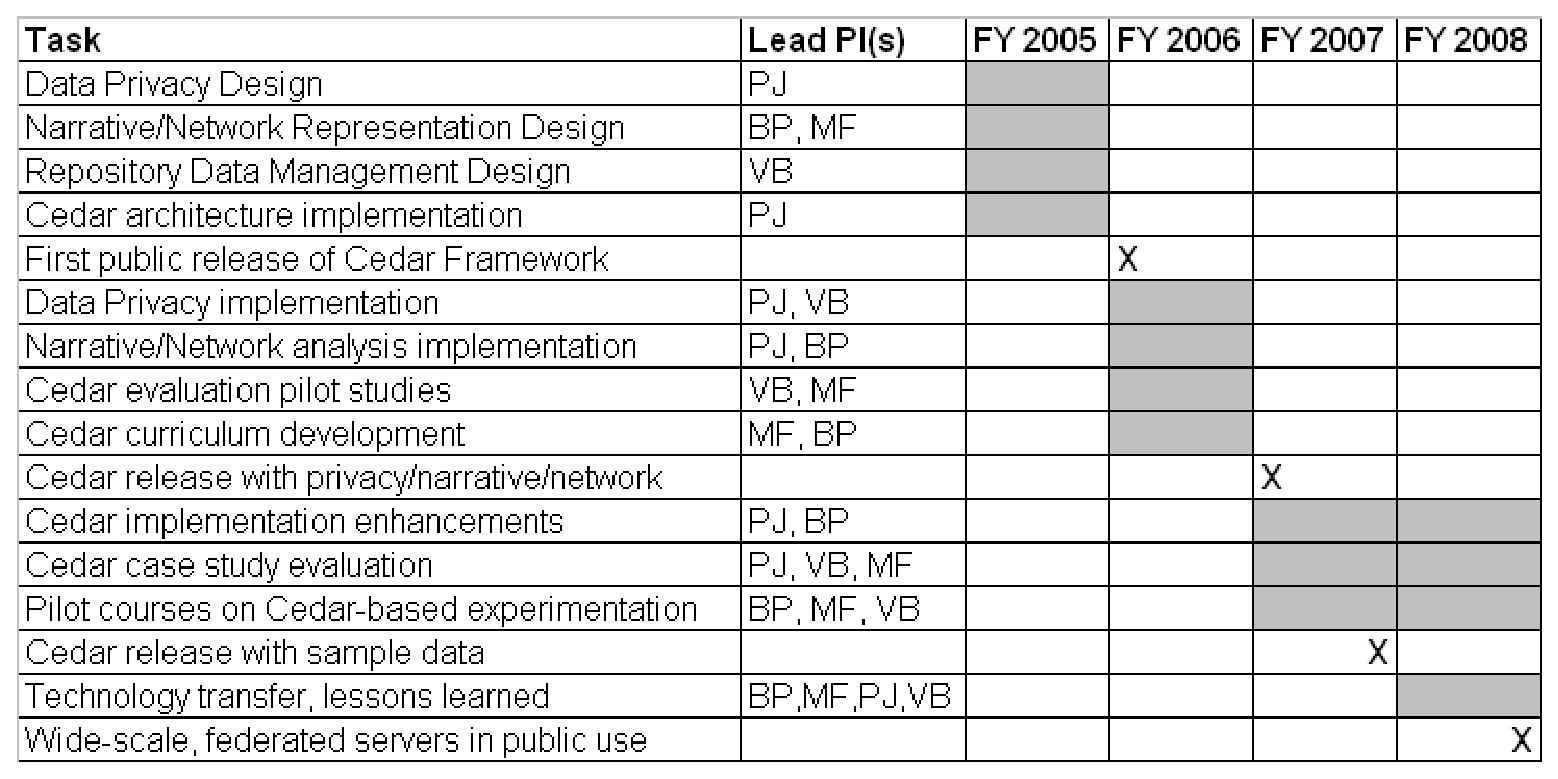
\includegraphics[width=0.75\textwidth]{workstructure.eps}
  \caption{Work breakdown structure and milestones}
  \label{fig:timeline}
\end{figure*}

Figure \ref{fig:timeline} outlines the major tasks, lead PI(s), and
milestones we have planned for this project.  Although all PIs will be in
close communication and involved with all aspects of the project, we
believe that some decoupling, particularly in the initial phase of the
project, will enable us to make progress more quickly.  

In the initial year, the primary tasks will be to design privacy policies,
narrative/network representations, and data repository management
mechanisms; and implement the architectural framework for Cedar. We will
also perform some ``pre-pilot'' case study work to validate our current
requirements and gather additional ones for deployment of Cedar into the
HPCS organization.  At the end of this initial year, we will make a public
release of our framework along with documents specifying the results of our
design activities.

In the second year, we will implement the designs developed during the
first year, and begin classroom case studies with Cedar which will result
in curriculum materials.  By half way through the funding period, at the
beginning of the third year, we plan to have a first release of the fully
functional Cedar cyberinfrastructure.

While we plan to continuously refine and improve the system for the
remainder of the grant period, this process will be driven by more
comprehensive evaluation activities during the second half of the grant
period, including pilot courses, case studies in the HPCS organization, and
external evaluation.  In the final year, we will begin effort on technology
transfer, developing documentation and training materials and conducting
tutorials as necessary to help broaden usage of Cedar.  By the end of the
grant period, we plan for a federated network of at least 50 to 100 Cedar
servers in active use, and that the success of this framework in the HPCS
community has created interest and involvement in the Cedar Consortium by
both academic and commercial organizations.

All of the PIs have extensive prior experience working in distributed
``virtual'' organizations, and we have learned how to be productive despite
geographical separation.  We will use a variety of synchronous and
asynchronous mechanisms to facilitate communication and coordination among
the Cedar research group. We plan to have a weekly teleconference meeting
between the PIs and graduate students to discuss tasks and challenges. Our
travel budgets include funds for on-site meetings twice a year for more
intensive, face-to-face interaction where we can review progress and
establish goals and milestones for the next six month period.  Finally, we
will provide a website similar to www.hackystat.org that will provide a
portal for access to source code, documentation, tech reports, wiki
collaboration, a public Cedar server, and so forth.

\subsection{Cedar in action}

To illustrate the benefits of Cedar, consider once again Figures
\ref{fig:dailydiary} and \ref{fig:telemetry}, which illustrate some of
quantitative data available about a high performance computing system
development project.  Effective interpretation and application of this
experience raises many questions : Are the trends in serial and parallel
code typical? Under what circumstances would a new development project
produce the same size trends? What are the strengths and weaknesses of the
chosen tool set (g++, mpiCC, etc.)?  Answering these questions requires
contextual, qualitative data, much of which is potentially available in
other artifacts associated with this study (the developer's engineering
logs, emails, and so forth).

One goal of Cedar is to provide an effective representation for tying the
quantitative to the qualitative, and it accomplishes this by supporting the
creation of a high-level abstract narrative, or ``story'' of this
development project which incorporates both the quantitative numbers and
the explanations for how the numbers came about.  In this case, some of the
relevent context is that the developer is a graduate student, was
implementing his first MPI program, was more concerned with functional
correctness than parallel speedup during this project, and encountered a
major requirements change in February 2005, leading to the sudden
perturbation in both parallel and serial code size. Such context is crucial
for assigning meaning to these numbers.

The narrative representation has another benefit beyond data integration:
it also provides a way for a user to query the federated network of Cedar
servers for similar ``stories''.  For example, having constructed this
narrative, one can then query the network to learn about other case studies
involving, for example, MPI software development.  The level of detail
provided back in response to this query will depend upon the privacy
policies in force related to each instance of the narrative. The
incremental generation of a collection of narratives, related in various
ways, creates a rich web of qualitative and quantitative data that provides
context for each single narrative as part of a larger community of
practice.






















%%%%%%%%%%%%%%%%%%%%%%%%%%%%%% -*- Mode: Latex -*- %%%%%%%%%%%%%%%%%%%%%%%%%%%%
%% project-contributions.tex -- 
%% Author          : Philip Johnson
%% Created On      : Thu Oct  4 08:05:31 2001
%% Last Modified By: Philip M. Johnson
%% Last Modified On: Wed May 25 13:15:26 2005
%% RCS: $Id$
%%%%%%%%%%%%%%%%%%%%%%%%%%%%%%%%%%%%%%%%%%%%%%%%%%%%%%%%%%%%%%%%%%%%%%%%%%%%%%%
%%   Copyright (C) 2001 Philip Johnson
%%%%%%%%%%%%%%%%%%%%%%%%%%%%%%%%%%%%%%%%%%%%%%%%%%%%%%%%%%%%%%%%%%%%%%%%%%%%%%%
%% 
\section{Conclusions}

We believe the Cedar project has substantial intellectual merit: it brings
together not only qualitative and quantitative data, but also researchers
from multiple disciplines to synthesize their knowledge and capabilities to
produce a system with unique capabilities.  The four Principle
Investigators in this project bring a diverse, but complementary set of
skills regarding qualitative and quantitative data collection and analysis;
software development; and empirical data repository management. Our
application of narrative and network theories to integrating empirical data
is both novel and promising, and our prior development of the Hackystat system 
enables us to jump-start the Cedar implementation.

We have designed the Cedar project with the intention that it be broadly
applicable as a tool for collecting, analyzing, and disseminating
qualitative and quantitative data.  As the University of Hawaii is a
university with 75\% minority students in an EPSCOR state, this project
will provide novel research opportunities to underrepresented groups. 
The development of curriculum materials, classroom evaluation, case studies 
in HPCS, and technology transfer through the Cedar Consortium will all result
in enhancements to infrastructure for research and education. 

We would like to conclude by noting that the ability to gather and access
data of this sort brings with it a duty to develop ways of interpreting
these data responsibly.  We have already pointed out that existing data
bases have been subject to misuse and misrepresentation.  People who are
marginal in society are particularly vulnerable to misinterpretation of
their actions.  Poor people, for instance, find a variety of ways of coping
with the lack of money that may make them look like irresponsible parents
or even criminals when neither may be the case \cite{Crampton01, Edin91,
Stack74}.  

%% As the use of data bases become even more widespread there will be more
%% times when in the course of normal events, people are asked to abstract
%% from a series of actions to a pattern that has a particular meaning.  The
%% ability to generalize from a series of actions to either an intent or a
%% predicted outcome is fraught with difficulty and must be tempered by a
%% connection to the context in which the person is taking the actions.  This
%% is particularly true when people are attempting to abstract across cultural
%% lines as the same action may have different meanings in different cultural
%% contexts.  As we have the ability to keep track of more and more things
%% (which is the intent of this proposal), being able to tell when action
%% should be taken and what actions should be taken will be more and more
%% important.

%% No matter how fine-grained and complete the data are, there are always
%% multiple ways in which these data add up to something that has meaning.
%% For instance, our credit card companies are already very good at taking the
%% specific purchases on an existing credit card and generalizing to "someone
%% has stolen this credit card number".  They are not always right, however,
%% and sometimes a person has just gone on a shopping spree.  Moreover, even
%% if the purchases don't fit the normal pattern and even if it turns out that
%% there is someone else using the credit card, it could be the spouse of the
%% credit card holder (whose last name, of course, may not be the same as the
%% credit card holder) and the use may be entirely legitimate.  Credit card
%% companies have learned to contact the customer to find out what is going
%% on.

%% Not only are there multiple ways to interpret anything, but there are also
%% multiple things happening at the same time. A waiter often serves more than
%% one table at a time.  Thus, when the waiter goes to the kitchen to pick up
%% a salad for one table, he may also pick up the desert for another table.
%% What may seem to be one action (going to the kitchen to pick up an order)
%% is actually two actions in two active performances. Pentland observed the
%% same thing in software support hot lines, where individual support
%% engineers could have as many as 60 open calls in their queue at one time
%% \cite{Pentland92}.  Identifying a solution for one customer may solve a
%% similar problem for other customers.  Such concurrency is an every day
%% event in most organizations.  Hiring routines overlap with training
%% routines or with budgeting routines.

An important goal of this research is to help people
incorporate, rather than bypass, context so that interpretations are
smarter.  Cedar will enable data analysts to identify some of the multiple
stories (or at least be aware of the multiple stories) and think about what
questions they need to ask and who they need to ask them of in order to
sort through which stories are more likely than others.  We view this
project as an opportunity not only to be more precise in the data we are
gathering but also as a way to incorporate the intrinsic diversity of
meanings in any set of actions.  If we succeed, this project will allow us
to make the complexity of life more accessible rather than to obscure it.



%%%%%%%%%%%%%%%%%%%%%%%%%%%%%%% -*- Mode: Latex -*- %%%%%%%%%%%%%%%%%%%%%%%%%%%%
%% project-nsfstuff.tex -- 
%% Author          : Philip Johnson
%% Created On      : Thu Oct  4 08:05:31 2001
%% Last Modified By: Philip M. Johnson
%% Last Modified On: Mon May 16 12:01:54 2005
%% RCS: $Id$
%%%%%%%%%%%%%%%%%%%%%%%%%%%%%%%%%%%%%%%%%%%%%%%%%%%%%%%%%%%%%%%%%%%%%%%%%%%%%%%
%%   Copyright (C) 2001 Philip Johnson
%%%%%%%%%%%%%%%%%%%%%%%%%%%%%%%%%%%%%%%%%%%%%%%%%%%%%%%%%%%%%%%%%%%%%%%%%%%%%%%
%% 
\newpage
\section{Excerpts from the NSF Solicitation}

We need to both ensure
that we are achieving the goals of this solicitation, as well as clearly
addressing the standard NSF review criteria.  To help us get there, the
next two sections provide copies of text from the solicitation that
we will need to keep in mind as we proceed.

\subsection{Solicitation Goals}
\label{sec:solicitation}

Some of the solicitation goals include:
\begin{enumerate}

\item The development of tools that facilitate the integration of
qualitative and quantitative information from heterogeneous sources,
multiple media, and/or multiple modes;

\item Investment in basic research that addresses the protection of the
confidentiality of respondents in computerized, widely accessible
databases; and

\item The development of incentives, standards and policies for collecting,
storing, archiving, accessing, and publishing research results using
organization-relevant information.

\item Testbed I. information collected on organizations from a variety of
heterogeneous, independently developed data sources, such as administrative
and survey data, temporal, spatial and image data or textual data. The goal
is to free users from having to locate the data sources, interact with each
data source in isolation, and manually combine data from multiple formats
and multiple sources. This could be achieved through the creation of new
and more accurate and efficient ways to collect, code and analyze
qualitative information from case studies, and other sources, and to enable
the linking of this information with repositories of quantitative data,
while protecting fundamental privacy and confidentiality concerns. The
research should be designed to show how appropriate cybertools can lead to
multiple advances in the empirical understanding of how organizations
emerge, develop, thrive or weaken.

\item Proposals must address the protection of data providers from
identification, exploitation, and other misuses of personal or
organizational information. Such misuses present a perpetual challenge to
the melding of data and media of different types in a tool for widespread
use. Proposals in response to this solicitation must show a sophisticated
understanding of this sociotechnical problem and must propose to advance
fundamental knowledge of effective privacy protections during the
development of the analytical tools and in their later use by various
research communities.

\item Proposals must demonstrate potential long-term sustainability,
usability, and impact. This could be achieved for the organizational
"testbed", for example, by documenting proposed collaboration with firms in
an industry, attracting support from foundations or developing replicable
incentive-compatible policies for collecting, storing, accessing, and
disseminating data while continuing to utilize and advance relevant
cybertechnology.

\item Unifying Data Models and System Descriptions: There is a need to
develop stronger theoretical foundations for the representation and
integration of information of various types from extant data models (e.g.,
temporal, spatial and image data, textual data, administrative and survey
data) as well as the scientific literature into conceptually coherent
views.

\item Reconciling heterogeneous formats schemas and ontologies: The
fundamental problem in any data sharing application is that systems are
heterogeneous in many different aspects, such as different ways of
representing data and/or knowledge about the world, different
representation mechanisms (e.g., relational databases, legacy systems, XML
schemas, ontologies), different access methods and policies. In order to
share data among heterogeneous sources, approaches to form a semantic
mapping of their respective representations are needed to avoid manual
intervention in each step of converting and merging data resources.

\item Web semantics: Data on the web needs to be defined and linked in a
way that it can be used by machines not just for display purposes, but also
for automation, integration and reuse of data across various
applications. Supported research topics will include frameworks for
describing resources, methods of automating inferences about web data and
resources, and the development of interoperable ontologies, mark up
languages and representations for specific social, behavioral and other
scientific domains.

\item Decentralized data-sharing: Traditional data integration systems use
a centralized mediation approach, in which a centralized mediator,
employing a mediated schema, accepts user queries and reformulates them
over the schemas of the different sources. However, mediated schemas are
often hard to agree upon, construct and maintain. For example, researchers
conducting social and behavioral research share their experimental results
with each other, but may do it in an ad hoc fashion. A similar scenario is
found in data sharing among government agencies. Architectures and
protocols that enable large-scale sharing of data with no central control
are needed.

\item On-the-fly integration: Currently, data integration systems rely on
relatively static configurations with a set of long-lived data
sources. On-the-fly integration refers to scenarios where one wants to
integrate data from a source immediately after discovering it. The
challenge is to significantly reduce the time and skill needed to integrate
data sources so that scientists can focus on domain problems instead of
information technology challenges.

\end{enumerate}

\subsection{NSF Review Guidelines}

The generic ones are:

\begin{enumerate}
\item What is the intellectual merit of the proposed activity?  How
important is the proposed activity to advancing knowledge and understanding
within its own field or across different fields? How well qualified is the
proposer (individual or team) to conduct the project? (If appropriate, the
reviewer will comment on the quality of the prior work.) To what extent
does the proposed activity suggest and explore creative and original
concepts? How well conceived and organized is the proposed activity? Is
there sufficient access to resources?

\item What are the broader impacts of the proposed activity?  How well does
the activity advance discovery and understanding while promoting teaching,
training, and learning? How well does the proposed activity broaden the
participation of underrepresented groups (e.g., gender, ethnicity,
disability, geographic, etc.)? To what extent will it enhance the
infrastructure for research and education, such as facilities,
instrumentation, networks, and partnerships? Will the results be
disseminated broadly to enhance scientific and technological understanding?
What may be the benefits of the proposed activity to society?

\item Integration of Research and Education One of the principal strategies
in support of NSF's goals is to foster integration of research and
education through the programs, projects, and activities it supports at
academic and research institutions. These institutions provide abundant
opportunities where individuals may concurrently assume responsibilities as
researchers, educators, and students and where all can engage in joint
efforts that infuse education with the excitement of discovery and enrich
research through the diversity of learning perspectives.

\item Integrating Diversity into NSF Programs, Projects, and Activities
Broadening opportunities and enabling the participation of all citizens --
women and men, underrepresented minorities, and persons with disabilities
-- is essential to the health and vitality of science and engineering. NSF
is committed to this principle of diversity and deems it central to the
programs, projects, and activities it considers and supports.

\end{enumerate}

There are several final review criteria specific to this solicitation:

\begin{enumerate}

\item  Possession of the scientific expertise and resources needed for tool development.
\item Possession of the scientific expertise and resources needed for the creation and analysis of databases on organizations and individuals.
\item  Cohesion of technology, tools and data within each "testbed".
\item  Documented outreach and dissemination plan.
\item Evidence of applicability to a broad range of sciences.
\item Quality of coordination plan.
\item Demonstration of scalability to, for example, additional organizations or other large-scale databases.
\item Evidence of long-term sustainability and impact.

\end{enumerate}
















\newpage
\bibliography{/export/home/csdl/bib/csdl-trs,nsf}
\bibliographystyle{plain}

%%%%%%%%%%%%%%%%%%%%%%%%%%%%%%% -*- Mode: Latex -*- %%%%%%%%%%%%%%%%%%%%%%%%%%%%
%% bio.tex -- 
%% Author          : Philip Johnson
%% Created On      : Tue Nov  4 10:26:48 1997
%% Last Modified By: Philip Johnson
%% Last Modified On: Thu Dec 10 14:58:10 2009
%% RCS: $Id$
%%%%%%%%%%%%%%%%%%%%%%%%%%%%%%%%%%%%%%%%%%%%%%%%%%%%%%%%%%%%%%%%%%%%%%%%%%%%%%%
%%   Copyright (C) 1997 Philip Johnson
%%%%%%%%%%%%%%%%%%%%%%%%%%%%%%%%%%%%%%%%%%%%%%%%%%%%%%%%%%%%%%%%%%%%%%%%%%%%%%%
%% 

%\section*{Biographical Sketch}
%\pagenumbering{arabic}
%\renewcommand{\thepage} {E--\arabic{page}}


%%      Command to define new categories:
\newcommand{\newcategory}[1]{\newenvironment{#1}
 {\sectionheading{#1}\begin{list}{}{\setlength{\labelwidth}{0cm} \setlength{\labelsep}{0cm} \setlength{\itemsep}{0ex plus0.2ex} \setlength{\itemindent}{-1cm} \setlength{\leftmargin}{1cm} \setlength{\parsep}{0ex plus0.2ex}}}{\end{list}\par}}

\newcommand{\sectionheading}[1]{\medskip\pagebreak[2]\par\noindent
 {\small\bf #1}\nopagebreak}

\begin{center}
Philip M. Johnson\\
Information and Computer Sciences \hfill (808) 956-3489

University of Hawaii              \hfill fax: (808) 956-3548

1680 East-West Road               \hfill johnson@hawaii.edu

Honolulu, HI~~~96822              \hfill http://philipmjohnson.org

\end{center}

\newcategory{Professional Preparation}
\begin{Professional Preparation}
\item Ph.D.~in Computer Science, University of Massachusetts. 1990 
\item M.S.~in Computer Science, University of Massachusetts.  1985
\item B.S.~in Biology, University of Michigan. 1980
\item B.S.~in Computer Science, University of Michigan. 1980
\end{Professional Preparation}

\newcategory{Appointments}
\begin{Appointments}
\item {\em Professor},  Information and Computer
  Sciences, University of Hawaii.  2001---present

\item {\em Visiting Professor}, School of Engineering, Blekinge Institute of Technology, Sweden, 2006.

\item {\em Associate Professor},  Information and Computer
  Sciences, University of Hawaii.  1995---2001

\item {\em Senior Research Fellow},  Distributed Systems Technology Centre,
University of Queensland, Australia, 1997.

\item {\em Assistant Professor},   Information and Computer
  Sciences, University of Hawaii.  1990---1995

\end{Appointments}




\newcategory{Products: Closely Related}
\begin{Products: Closely Related}

\item R.Brewer, Y. Xu, G. Lee, M. Katchuck, C. Moore, P. Johnson, {\em Three principals for the design of energy feedback visualizations}, International Journal on Advances in Intelligent Systems,Volume 6, No. 3, December 2013.


\item R. Brewer, Y. Xu, G. Lee, M. Katchuck, C. Moore, P. Johnson, {\em Energy feedback for smart grid consumers: Lessons learned from the Kukui Cup}, Proceedings of Energy 2013, Lisbon, Portugal, March 2013.


\item P. Johnson, Y. Xu, R. Brewer,  C. Moore,  G. Lee, A. Connell, {\em Makahiki+WattDepot: An open source software stack for next generation energy research and education}, Proceedings of the 2012 Conference on Information and Communication Technologies for Sustainability, Zurich, Switzerland, February 2013.

\item P. Johnson, Y. Xu, R. Brewer, G. Lee, M. Katchuck, C. Moore, {\em Beyond kWh: Myths and fixes for energy competition game design}, Proceedings of Meaningful Play 2012, Lansing, Michigan, October 2012.

\item R. Brewer and P. Johnson, {\em WattDepot: An open source software ecosystem for enterprise-scale energy data collection, storage, analysis, and visualization}, Proceedings of the First IEEE International Conference on Smart Grid Communications, Gaithersburg, Maryland, October 2010.


\end{Products: Closely Related}


\newcategory{Products: Other Significant}
\begin{Products: Other Significant}

\item H. Kou and P. Johnson and H. Erdogmus, {\em Operational Definition and 
Automated Inference of Test-Driven Development with Zorro}, 
Journal of Automated Software Engineering, December, 2009.

\item P. Johnson and S. Zhang, {\em We need more coverage, stat!  Experiences with the Software ICU}, 
Proceedings of  Empirical Software Engineering and Measurement, October, 2009.
  
\item V. Basili and M. Zelkowitz and D. Sjoberg and P. Johnson and T. Cowling,
{\em Protocols in the use of Empirical Software Engineering Artifacts}, 
Empirical Software Engineering, Volume 12, February, 2007.

\item P. Johnson, {\em Requirement and Design Trade-offs in Hackystat: An
in-process software engineering measurement and analysis system},
Proceedings of the 2007 International Symposium on Empirical Software
Engineering and Measurement, Madrid, Spain, September, 2007.

\item L. Hochstein and T. Nakamura and V. Basili and S. Asgari and 
M. Zelkowitz and J. Hollingsworth and F. Shull and J. Carver and 
M. Voelp and N. Zazworka and P. Johnson, {\em Experiments to 
understand HPC time to development}, CTWatch Quarterly, 
November, 2006.

\end{Products: Other Significant}


\newcategory{Synergistic Activities}
\begin{Synergistic Activities}

\item {Project Leader}, Open Power Quality, http://openpowerquality.org/

\item {Project Leader}, Kukui Cup, http://kukuicup.org/

\item {Project Leader}, Hackystat Framework, http://www.hackystat.org/

\end{Synergistic Activities}

\renewcommand{\newcategory}[1]{\newenvironment{#1}
 {\sectionheading{#1}\begin{list}{}{\setlength{\labelwidth}{0cm} \setlength{\labelsep}{0cm} \setlength{\itemsep}{0ex plus0.2ex} \setlength{\itemindent}{0cm} \setlength{\leftmargin}{0cm} \setlength{\parsep}{0ex plus0.2ex}}}{\end{list}\par}}


\newcategory{Collaborators and other affiliations}
\begin{Collaborators and other affiliations}
\item {\em Collaborators and Co-Editors.} 
Victor Basili (University of Maryland),
Jeff Carver (University of Alabama),
Hackan Erdogmus (National Research Council, Canada), 
Stuart Faulk (University of Oregon),
Brian Pentland (Michigan State University),
Dan Port (University of Hawaii),
Forrest Shull (Fraunhofer-Maryland),
Larry Votta (Sun Microsystems),
Claes Wohlin (Blekinge Institute of Technology, Sweden),
Marvin Zelkowitz (University of Maryland).
Total collaborators and co-editors: 10.
\medskip

\item {\em Graduate Advisors and Postdoctoral Sponsors.} 
Jack Wileden, Wendy Lehnert, Victor Lessor (all University of Massachusetts).  Postdoctoral sponsor: none.  Total graduate advisors and postdoctoral sponsors: 3.
\medskip

\item {\em Thesis Advisor and Postgraduate-Scholar Sponsor}. 
Robert Brewer (Ph.D. 2013, Aarhus University),
Anthony Christe (Ph.D. student),
%Monir Hodges,
%Aaron Kagawa, 
%Hongbing Kou,
%Christoph Lofi,
Carleton Moore (Ph.D. 2000, University of Hawaii),
%Mette Moffett, 
Sergey Negrashov (Ph.D. student),
%Alexey Olkov, 
%Michael Paulding,
Pavel Senin (Ph.D. 2015, INRA MIA),
%Danu Tjahjono,
%Dadong Wan,
Yongwen Xu (Ph.D. student), 
%Takuya Yamashita,
%Cedric Zhang, 
%Shoaxuan Zhang. 
Total graduate students advised and postdoctoral scholars sponsored: 18
\end{Collaborators and other affiliations}








%%%%%%%%%%%%%%%%%%%%%%%%%%%%%%% -*- Mode: Latex -*- %%%%%%%%%%%%%%%%%%%%%%%%%%%%
%% budget.tex -- 
%% Author          : Philip Johnson
%% Created On      : Wed Jul 27 13:31:23 1994
%% Last Modified By: Philip M. Johnson
%% Last Modified On: Mon Jun 13 11:02:17 2005
%% Status          : Unknown
%% RCS: $Id$
%%%%%%%%%%%%%%%%%%%%%%%%%%%%%%%%%%%%%%%%%%%%%%%%%%%%%%%%%%%%%%%%%%%%%%%%%%%%%%%
%%   Copyright (C) 1994 University of Hawaii
%%%%%%%%%%%%%%%%%%%%%%%%%%%%%%%%%%%%%%%%%%%%%%%%%%%%%%%%%%%%%%%%%%%%%%%%%%%%%%%
%% 

\documentclass[11pt]{article} 
\usepackage{/export/home/csdl/tex/icse2003/latex8}
\usepackage{times}
\usepackage[final]{graphicx}
% uncomment the % away on next line to produce the final camera-ready version
% and uncomment the \thispagestyle{empty} following \maketitle
%\pagestyle{empty}



\begin{document}


\pagestyle{empty}
\section*{Budget Justification}

\subsection*{Salaries}

The project budget provides salary support for the principal investigator
(two summer months) and two graduate research
assistants (11 months) for each of the three years.  The principal
investigator will perform or supervise all major system design enhancements
and empirical studies, manage and train the graduate student
assistants, and supervise case studies. 

\subsection*{Travel}

The project budget provides funds for two trips per year from Hawaii to the
mainland.  These trips will be used to attend
relevant conferences (e.g., ICSE, FSE, ISERN, or STAR), where
he may report on the results of his own work and obtain first hand
information on related work. 

\subsection*{Computer Services}

The principal investigator directs the Collaborative Software Development
Laboratory, which is currently equipped with one enterprise SUN server and
8 workstations, along with a printer and networking
peripherals.  The project budget provides funds of \$10,000/year to 
provide workstations and associated software for the principal investigator and 
the two graduate research assistants. In addition, these funds will maintain 
a server for the public Hackystat site and the developer services site. 

\subsection*{Cost breakdown}
\label{cost-breakdown}

All calculations are rounded to the nearest dollar.

\paragraph{Summer Salary.}  
Summer salary is calculated as two additional months of the principal
investigator's annual nine month salary.  Summer salary includes the pay
increases as negotiated through collective bargaining.  Pay increases are
as follows: 5\% in 2006 (year 1), 9\% in 2007 (year 2) and 11\% in 2008
(year 3).
 

\paragraph*{Research Assistants.}  
This cost category provides support for two graduate research assistants
for each of the four years.  The salary for each research assistant is
based upon RA-Step 3.

\paragraph*{Fringe benefits.} 
Fringe benefits for salaries are calculated at 3.5\% for the principal
investigator and 25\% for the graduate assistants.

\paragraph*{Overhead.}  
University of Hawaii overhead cost is calculated as 36.3\% of Modified Total
Direct Costs (MTDC), i.e. salaries, travel, and supplies (equipment is
excluded).





\end{document}


\end{document}








